% % % % % % % %  MDT UFSM 2021  % % % % % % % % 
%% Arquivo base para o documento - ver. 1.0 %%
% % % % % % % % % % % % % % % % % % % % % % % % 


% % % OPCOES DE COMPILACAO
% % % PAGINACAO
% % % PAGINACAO SIMPLES (FRENTE): PARA TRABALHOS COM MENOS DE 100 PAGINAS
\documentclass[oneside,openright,12pt]{ufsm_2021} %%%%% OPCAO PADRAO -> PAGINACAO SIMPLES. PARA TRABALHOS COM MAIS DE 100 PAGINAS COMENTE ESTA LINHA E DESCOMENTE A LINHA 
% % % % % % % % % % % % % % % % % % % % % % % % % % % % % % % % % % % % % % %
% PAGINACAO DUPLA (FRENTE E VERSO): PARA TRABALHOS COM MAIS DE 100 PAGINAS
% \documentclass[twoside,openright,12pt]{ufsm_2021}  %%%% PARA TRABALHOS COM MAIS DE 100 PAGINAS DESCOMENTE AQUI
% % % % % % % % % % % % % % % % % % % % % % % % % % % % % % % % % % % % %




% % % %  CODIFICACAO DO TEXTO 
% % % %  POR PADRAO USA-SE UTF8. PARA APLICAR A CODIFICACAO OESTE EUROPEU (ISO 8859-1) DESCOMENTE A LINHA ABAIXO. ELA ATIVA A OPCAO "latin1" DO PACOTE "inputenc"
% \oesteeuropeu
% % % % % % % % % % % 



% % % % % % % % PACOTES PESSOAIS % % % % % % % %  
\usepackage{lipsum}
\usepackage{quoting}


% % % % % % % % DEFINICOES PESSOAIS % % % % % % % %







% % % % % % % % % % % % % % % % % % % % % % % % % % % % % % % % % % % % % % % % % % % 




% % % % % % % % % % % % % % % % % % % % % % % % % % % % % % % % % 
% % % % % % % % % % % % DADOS DO TRABALHO % % % % % % % % % % % % 
% % % % % % % % % % % % % % % % % % % % % % % % % % % % % % % % % 

% % % % % % % % % % INFORMACOES INSTITUCIONAIS % % % % % % % % % % 


% % CENTRO DE ENSINO DA UFSM
\centroensino{Colégio Politécnico}  %%% NOME POR EXTENSO
\centroensinosigla{CP}  %%% SIGLA

% % CURSO DA UFSM
\nivelensino{Graduação}  %%%%%%% NIVEL DE ENSINO 
\curso{Sistemas Para Internet}   %%%%% NOME POR EXTENSO 
\ppg{PPGALGO}   %%%%%% SIGLA
\statuscurso{Curso}  %%%% STATUS= {Programa} ou {Curso}
% \EAD  %%%% para cursos EAD
% % % %  LOCAL DO CAMPUS OU POLO
\cidade{Santa Maria}
\estado{RS}


% % % % % % % % % % INFORMACOES DO AUTOR % % % % % % % % % % 
\author{Pedro Hasan Carara}   %%%%% AUTOR DO TRABALHO
\sexo{M} %%%% SEXO DO AUTOR -> M=masculino   F=feminino (IMPORTANTE PARA AJUSTAR PAGINAS PRE-TEXTUAIS)
\grauensino{graduação}    %%%%%%%% GRAU DE ENSINO A SER CONCLUIDO
\grauobtido{Tecnólogo}    %%%%% TITULO OBTIDO
\email{cararax@gmail.com}   %%%% E-MAIL PARA CATALOGRAFICA (COPYRIGHT) - OBRIGATORIO
%\endereco{Rua das abobrinhas, n. 666} %%%% TELEFONE PARA CATALOGRAFICA (COPYRIGHT) (CAMPO OPICIONAL -- CASO NAO POSSUA OU NAO QUEIRA DIVULGAR COMENTE A LINHA)
%\fone{11 2222 3333}   %%%% TELEFONE PARA CATALOGRAFICA (COPYRIGHT) FORMATO {11 2222 3333} (CAMPO OPICIONAL -- CASO NAO POSSUA OU NAO QUEIRA DIVULGAR COMENTE A LINHA)
%\fax{11 2222 3333}   %%%% FAX PARA CATALOGRAFICA (COPYRIGHT) FORMATO {11 2222 3333} (CAMPO OPICIONAL -- CASO NAO POSSUA OU NAO QUEIRA DIVULGAR COMENTE A LINHA)


% % % % % % % % % % INFORMACOES DA BANCA % % % % % % % % % % 
% OBSERVACOES: O CAMPO ORIENTADOR EH OBRIGATORIO E NAO DEVE SER COMENTADO

\orientador{Daniel Lichtnow}{Dr}{UFSM}{M}{P}  %%%INFORMACOES SOBRE ORIENTADOR: OS CAMPOS SAO:{NOME}{SIGLA DA TITULACAO}{SIGLA DA INSTITUICAO DE ORIGEM}{SEXO} M=masculino   F=feminino {PARTE DA BANCA?} P=presidente  M=Membro  N=Nao faz parte
%\coorientador{Co-orientador}{Dra}{AAAA}{F}{M} %%%INFORMACOES SOBRE CO-ORIENTADOR: OS CAMPOS SAO:{NOME}{SIGLA DA TITULACAO}{SIGLA DA INSTITUICAO DE ORIGEM}{SEXO} M=masculino   F=feminino {PARTE DA BANCA?} P=presidente  M=Membro  N=Nao faz parte
\bancaum{Rafael Gressler Milbradt}{Dr}{UFSM}{M}{M}  %%%INFORMACOES SOBRE PRIMEIRO NOME DA BANCA: OS CAMPOS SAO:{NOME}{SIGLA DA TITULACAO}{SIGLA DA INSTITUICAO DE ORIGEM}{SEXO} M=masculino   F=feminino {PARTE DA BANCA?} P=presidente  M=Membro  N=Nao faz parte
\bancadois{Vinícius Maran}{Dr}{UFSM}  %%%INFORMACOES SOBRE SEGUNDO NOME DA BANCA: OS CAMPOS SAO:{NOME}{SIGLA DA TITULACAO}{SIGLA DA INSTITUICAO DE ORIGEM}
% \bancatres{Banca Três}{Dra}{CCCC} %%%INFORMACOES SOBRE TERCEIRO NOME DA BANCA: OS CAMPOS SAO:{NOME}{SIGLA DA TITULACAO}{SIGLA DA INSTITUICAO DE ORIGEM}
% \bancaquatro{Banca Quatro}{Dr}{DDDD} %%%INFORMACOES SOBRE QUARTO NOME DA BANCA: OS CAMPOS SAO:{NOME}{SIGLA DA TITULACAO}{SIGLA DA INSTITUICAO DE ORIGEM}
% \bancacinco{Banca Cinco}{Dra}{EEEE} %%%INFORMACOES SOBRE QUARTO NOME DA BANCA: OS CAMPOS SAO:{NOME}{SIGLA DA TITULACAO}{SIGLA DA INSTITUICAO DE ORIGEM}
% \supervisor{Al Paccino}{Dr}{MAFIA}{M}{N} %%%INFORMACOES SOBRE SUPERVISOR (indicado para estagios): OS CAMPOS SAO:{NOME}{SIGLA DA TITULACAO}{SIGLA DA INSTITUICAO DE ORIGEM}{SEXO} M=masculino   F=feminino {PARTE DA BANCA?} P=Presidente  M=Membro  N=Nao faz parte



% % % % % % % % % % REALIZACAO POR VIDEO CONFERENCIA (MEMORANDO 04/2016 BIBLIOTECA CENTRAL UFSM)
\videoconferencia % % % % QUANDO O ACADEMICO DEFENDE POR VIDEO CONFERENCIA (PERMITIDO PELO ARTIGO 82 DO REGIMENTO GERAL DA PRPGP/UFSM). PARA DEFESAS NAS QUAIS O ACADEMICO ESTA PRESENTE COMENTE ESTA LINHA
% % % % QUANDO UM DOS MEMBROS DA BANCA PARTICIPA POR VIDEO CONFERENCIA INDICAR O MEMBRO DE ACORDO COM A LISTA ABAIXO. CASO CONTRARIO MANTER A PALAVRA "NAO". SAO PERMITIDOS, PELO REGIMENTO PRGPGP (ARTIGO 83) ATE 2 MEMBROS 
\videoconferenciabancap{NAO}  %%%% PRIMEIRO MEMBRO
\videoconferenciabancas{NAO}  %%%%% SEGUNDO MEMBRO
% % O > ORIENTADOR
% % CO > COORIENTADOR% % % % QUANDO UM DOS MEMBROS DA BANCA PARTICIPA POR VIDEO CONFERENCIA INDICAR O MEMBRO DE ACORDO COM A LISTA ABAIXO. CASO CONTRARIO MANTER A PALAVRA "NAO". SAO PERMITIDOS, PELO REGIMENTO PRGPGP ATE 2 MEMBROS.
% % 1 > BANCA UM
% % 2 > BANCA DOIS
% % 3 > BANCA TRÊS
% % 4 > BANCA QUATRO
% % 5 > BANCA CINCO
% % S > SUPERVISOR
% % % % % % % % % % % % % % % % % % % % % % % % % % % % % % % % % % % % 



% % % % % % % % % % INFORMACOES SOBRE O TRABALHO % % % % % % % % % %
% % % %  TITULO E SUBTITULO DO TRABALHO: ELES NÃO DEVEM ULTRAPASSAR, JUNTOS, 3 LINHAS NA COMPILAÇÃO DA CAPA. 
% SE O TRABALHO POSSUI SUBTITULO, ADICIONE ':' DENTRO DAS CHAVES ABAIXO 
\titulo{Microsserviços e bancos de dados} %% NAO EH NECESSARIO CAPITALIZAR
% % % %  TITULO DO TRABALHO EM INGLES
% SE O TRABALHO POSSUI SUBTÍTULO, ADICIONE ':' DENTRO DAS CHAVES ABAIXO 
\englishtitle{Microservices and databases}  %% NAO EH NECESSARIO CAPITALIZAR


% % % % O SUBTÍTULO É OPCIONAL, SE NÃO FOR USADO AS LINHAS ABAIXO DEVEM SER COMENTADAS

% SE O TRABALHO POSSUI SUBTÍTULO, ADICIONE ':' DENTRO DAS CHAVES ABAIXO 
%\subtitulo{Subtítulo do trabalho em português} %% NAO EH NECESSARIO CAPITALIZAR
% % % %  SUB TITULO DO TRABALHO EM INGLES
%\subenglishtitle{Subtítulo do trabalho em inglês}  %% NAO EH NECESSARIO CAPITALIZAR

% % % AREA DE CONCENTRACAO DO TRABALHO (CNPQ)
\areaconcentracao{Ciências Exatas e da Terra}
% % % TIPO DE TRABALHO - MANTER APENAS UMA LINHA DESCOMENTADA
\tese  %% Tese de <nivel de ensino>
% \qualificacao %% Exame de Qualificação de <nivel de ensino>
% \dissertacao %% Dissertacao de <nivel de ensino>
% \monografia %% Monografia
% \monografiag  %% Monografia (nao exibe area de concentracao)
% \tf  %% Trabalho Final de <nivel de ensino>
% \tfg  %% Trabalho Final de Graduacao (nao exibe area de concentracao)
% \tcc  %% Trabalho de Conclusao de Curso
% \tccg  %% Trabalho de Conclusao de Curso (nao exibe area de concentracao)
% \relatorio  %% Relatório de Estágio (nao exibe area de concentracao)
% \generico   %%% Alternativa para aqueles cursos que nao recebem o titulo de bacharel ou licenciado. Ex: engenharia, arquitetura, etc... Os campos abaixo tambem devem ser preenchidos
%     \tipogenerico{Tipo de trabalho em português}
%     \tipogenericoen{Tipo de trabalho em inglês}
%     \concordagenerico{o}
%     \graugenerico{Engenheiro Eletricista}
% % % DATA DA DEFESA 
\data{18}{08}{2024} %% FORMATO {DD}{MM}{AAAA}



% % % % %  ALGUMAS ENTRADAS PRE-TEXTUAIS
% % % % CASO NAO QUEIRA UTILIZA-LAS COMENTE A LINHA DE COMANDO
% % % EPIGRAFE
% \epigrafe{Winter is coming!}{Família Stark} %ESTRUTURA DE CAMPOS -> {Texto}{Autor}
% % % DEDICATORIA
% \dedicatoria{Aos que virão depois de nós}
% % % %  AGRADECIMENTOS
% \agradecimentos{A mim!}

% % % % %  RESUMO E PALAVRAS CHAVE DO RESUMO - OBRIGATORIO PARA MDT-UFSM
\resumo{
Este trabalho aborda a integração de bancos de dados com arquiteturas de microsserviços, explorando os desafios e soluções relacionados à consistência, disponibilidade e particionamento de dados. A arquitetura de microsserviços, caracterizada pela decomposição de uma aplicação em serviços pequenos e independentes, oferece vantagens em termos de escalabilidade, flexibilidade e resiliência. No entanto, a gestão de dados em um ambiente distribuído apresenta desafios como fragmentação de dados, consistência eventual, transações distribuídas e sincronização de dados. Para enfrentar esses desafios, o estudo analisa padrões de arquitetura como CQRS, Saga, Circuit Breaker e Event Sourcing, avaliando suas vantagens e desvantagens. A aplicação fictícia "ReservaExpress" será utilizada como estudo de caso para ilustrar a implementação desses padrões, com o uso de ferramentas e frameworks que facilitam a implementação de padrões de microsserviços, como o Axon Framework.

% Escreva seu resumo aqui! Você pode digitá-lo diretamente neste arquivo ou usar o comando input. O resumo deve ter apenas uma página, desde o cabeçalho até as palavras chave. Caso seu resumo seja maior, use comandos para diminuir espaçamento e fonte (até um mínimo de 10pt) no texto.  Segundo a MDT, é preciso que os resumos tenham, no máximo, 250 palavras para trabalhos de conclusão de curso de graduação, pós-graduação e iniciação científica e até 500 palavras para dissertações e teses.
}
\palavrachave{Microsserviços; Bancos de Dados; CQRS; Saga; Event Sourcing; Circuit Breaker.}
% "... deverão constar, no mínimo, três palavras-chave, iniciadas em
% letras maiúsculas, cada termo separado dos demais por ponto, e
% finalizadas também por ponto." MDT 2012

% % % % %  ABSTRACT E PALAVRAS CHAVE DO RESUMO - OBRIGATORIO PARA MDT-UFSM
\abstract{
This work addresses the integration of databases with microservices architectures, exploring the challenges and solutions related to data consistency, availability, and partitioning. Microservices architecture, characterized by the decomposition of an application into small and independent services, offers advantages in terms of scalability, flexibility, and resilience. However, data management in a distributed environment presents challenges such as data fragmentation, eventual consistency, distributed transactions, and data synchronization. To address these challenges, the study analyzes architectural patterns such as CQRS, Saga, Circuit Breaker, and Event Sourcing, evaluating their advantages and disadvantages. The fictitious application "ReservaExpress" will be used as a case study to illustrate the implementation of these patterns, using tools and frameworks that facilitate the implementation of microservices patterns, such as the Axon Framework.

% Write your abstract here! As recomendações do resumo também se aplicam ao abstract. \lipsum[0-1]
}
\keywords{Microservices; Databases; CQRS; Saga; Event Sourcing; Circuit Breaker}


% % %  ATIVACAO DE LISTAS E PAGINAS ESPECIAIS
% % %  PARA QUE APARECAO NAO NO TEXTO DESCOMENTE A LINHA ABAIXO -> POR PADRAO TODAS ESTAO ATIVIDADAS

% % LISTA DE FIGURAS 
% \semfiguras   %%(QUANDO ATIVIDA NAO EXIBE A LISTA)
% % LISTA DE GRAFICOS 
\semgraficos   %%(QUANDO ATIVIDA NAO EXIBE A LISTA)
% % LISTA DE ILUSTRACOES 
\semilustracoes  %%(QUANDO ATIVIDA NAO EXIBE A LISTA)
% % LISTA DE TABELAS 
%% \semtabelas   %%(QUANDO ATIVIDA NAO EXIBE A LISTA)
% % LISTA DE QUADROS 
\semquadros   %%(QUANDO ATIVIDA NAO EXIBE A LISTA)
% % LISTA DE APENDICES 
\semapendices  %%(QUANDO ATIVIDA NAO EXIBE A LISTA)
% LISTA DE ANEXOS 
\semanexos   %%(QUANDO ATIVIDA NAO EXIBE A LISTA)


% % % %  LISTA DE ABREVIATURAS - AMBIENTE TABULAR
%%%%%%%% para não utilizar comente as linhas abaixo.
% \abreviaturamax{SIGLAMAX} %%%% coloque aqui a maior sigla (indentacao)
% \listadeabreviaturas{
% 	SIGLA1 & Nome Completo da Sigla 1 \\
% 	SIGLA2 & Nome Completo da Sigla 2 \\
% 	SIGLAMAX &	Nome Completo da Sigla MAX \\
% }


% % % %  LISTA DE SIGLAS - AMBIENTE TABULAR
%%%%%%%% para não utilizar comente as linhas abaixo.
% \siglamax{SIGLAMAX} %%%% coloque aqui a maior sigla (indentacao)
% \listadesiglas{
% SIGLA1 & Nome Completo da Sigla 1 \\
% SIGLA2 & Nome Completo da Sigla 2 \\
% SIGLAMAX &	Nome Completo da Sigla MAX \\
% }


% % % %  LISTA DE SIMBOLOS
%%%%%%%% OBS: O espaco entre colchetes \item[] e um ambiente matematico
%%%%%%%% para não utilizar comente as linhas abaixo.
% \simbolomax{(Re)2} %%%% coloque aqui o maior simbolo (indentacao)
% \listadesimbolos{
% \item[u_*]	Escala de velocidade de fricção	
% \item[w_*]	Escala de velocidade convectiva
% \item[(Re)^2]	Maior simbolo da lista
% }


% % % FICHA CATALOGRAFICA
% \semcatalografica  %%%%  (QUANDO ATIVIDA NAO EXIBE A FICHA CATALOGRAFICA NECESSITA DO ARQUIVO DA FICHA: ficha_catalografica.pdf
% % % A FICHA CATALOGRAFICA FORNECIDA PELA UFSM EH UM PDF DO TAMANHO A4
% % % EH POSSIVEL GERA-LA NO SITE http://cascavel.ufsm.br/ficha_catalografica/
% % % OS COMANDOS ABAIXO DEFINEM AS MARGENS PARA CORTAR A FICHA FORNECIDA E COLOCA-LA COMO UMA FIGURA NO DOCUMENTO LATEX
\margemesquerda{1.9}   %%%% CORTE DE MARGEM ESQUERDA EM CM
\margemdireita{1.5}   %%%% CORTE DE MARGEM DIREITA EM CM
\margemsuperior{2.75}  %%%% CORTE DE MARGEM SUPERIOR EM CM
\margeminferior{2.9} %%%% CORTE DE MARGEM INFERIOR EM CM
% % %  DICA: IMPRIMA UMA COPIA DA FICHA CATALOGRAFICA E FACA A MEDIDA DAS MARGENS!





% % FOLHA DE ERRATA (versao rudimentar...pode ser aprimorado)
% % para não utilizar comente as linhas abaixo.
% % deve ser preenchida como um ambiente tabular de quatro colunas:
% % pagina & linha & onde se le & leia-a se \\
% \errata{
% 10   &    10    & errado   & certo \\
% \hline
% 12    &    5     & errado com um texto mais longo & certo agora com um texto mais longo\\
% \hline
% 13   &    3    & $x^2$   & $2x$\\
% }
% % % % % % % % % % % % % % % % % % % % % % % % % % % % % % % % % % % % % % % % % % % % % % 


% % % % % % % % % % % % % % % % % % % % % % % % % % % % % % % % % % % % % % 
% % % % % % % % % % % %  OPCOES DE FORMATACAO % % % % % % % % % % % % % % %
% % % % % % % % % % % % % % % % % % % % % % % % % % % % % % % % % % % % % % 
% % % CAPITULO: por padrao alinhado a esquerda. Para ativar alinhamento centralizado descomente o comando abaixo

% \centralizado  %%%% <<< centraliza todos os capitulos

% % % % % % % % % % % % % % % % % % % % % % % % % % % % % % % % % % % % % %
% % % FONTES: descomente uma das opcoes. caso nenhuma seja ativada a clase usara a fonte padrao do latex

% %% helvetica
% \usepackage[scaled]{helvet}
% \renewcommand*\familydefault{\sfdefault}

% arial
\renewcommand{\rmdefault}{phv} % Arial
\renewcommand{\sfdefault}{phv} % Arial

%%times
% \usepackage{mathptmx}

% % % % % % % % % % % % % % % % % % % % % % % % % % % % % % % % % % % % % % 
% % % % % % % % % % % % % % % % % % % % % % % % % % % % % % % % % % % % % % 
% % % % % % % % % % % % % % % % % % % % % % % % % % % % % % % % % % % % % % 
% % % % % % % % % % % % % % % % % % % % % % % % % % % % % % % % % % % % % % 


% % % % % % % % % % % % % % % % % % % % % % % % % % % % % % % % % % % % % % 
% % % % % % % % % % % % % % % % % % % % % % % % % % % % % % % % % % % % % % 
% % % % % % % % % % % %  INICIO DO DOCUMENTO  % % % % % % % % % % % % % % %
% % % % % % % % % % % % % % % % % % % % % % % % % % % % % % % % % % % % % % 
% % % % % % % % % % % % % % % % % % % % % % % % % % % % % % % % % % % % % %


\begin{document}



% % % % % % % % % % % % % % % % % % % % % % % % % % % % % % % % % % % % % % 
\pretextual  %%%% GERA AS PAGINAS PRE-TEXTUAIS   
% % % % % % % % % % % % % % % % % % % % % % % % % % % % % % % % % % % % % % 

% % % % % % % % % % % % % % % % % % % % % % % % % % % % % % % % % % % % % % 
% % % % % CORPO DO TRABALHO - INCLUA OS SEUS TEXTOS AQUI
% % % % % SUGESTAO -> UTILIZE ARQUIVOS EXTERNOS A PARTIR DO COMANDO \input
% % % % % % % % % % % % % % % % % % % % % % % % % % % % % % % % % % % % % % 
% % % % % % % % % % INICIO DAS PAGINAS TEXTUAIS % % % % % % % % % % % % % % 
% % % % % % % % % % % % % % % % % % % % % % % % % % % % % % % % % % % % % % 

% \chapter{Introdução}
% \par Insira aqui a introdução!!!
% \cite{richardson2018}
\chapter{Introdução}

A evolução dos sistemas de software ao longo das últimas décadas tem sido marcada por uma crescente complexidade e pela necessidade de maior flexibilidade e escalabilidade. Tradicionalmente, os sistemas monolíticos dominavam o cenário, caracterizados por uma única base de código e uma forte interdependência entre seus componentes. Contudo, com o aumento da demanda por desenvolvimento ágil e resposta rápida às mudanças do mercado, a arquitetura de microsserviços emergiu como uma alternativa eficaz.

Microsserviços são uma abordagem arquitetônica que estrutura uma aplicação como um conjunto de serviços pequenos e independentes, cada um executando uma funcionalidade específica. Essa abordagem permite que diferentes partes da aplicação sejam desenvolvidas, implantadas e escaladas de forma independente, promovendo uma maior agilidade e resiliência do sistema \cite{newman2019}.

Nesse contexto, os bancos de dados desempenham um papel crucial. Eles são responsáveis pelo armazenamento e recuperação dos dados que suportam as operações dos microsserviços. A transição para uma arquitetura de microsserviços implica em novos desafios para a gestão dos dados, uma vez que a abordagem tradicional de um único banco de dados centralizado pode não ser adequada para a natureza distribuída e independente dos microsserviços \cite{richardson2018}.

\section{Questão de Pesquisa}

A integração de bancos de dados com arquiteturas de microsserviços apresenta uma série de desafios. Entre eles, destacam-se a necessidade de garantir a consistência dos dados, a manutenção da disponibilidade e a adequação do particionamento dos dados. Esses desafios são exacerbados pela natureza distribuída dos microsserviços, onde cada serviço pode ter suas próprias necessidades de dados e requisitos de performance.

Portanto, a questão central desta pesquisa é: Quais são os principais desafios enfrentados na integração de bancos de dados com arquiteturas de microsserviços e quais são as soluções mais eficazes para superá-los? Especificamente, a pesquisa busca responder como garantir a consistência, a disponibilidade e o particionamento adequado dos dados em um ambiente de microsserviços.

Os desafios da integração de bancos de dados com microsserviços podem ser mitigados através de padrões arquiteturais bem estabelecidos. O SAGA e o Event Sourcing são fundamentais para manter a consistência dos dados, permitindo um controle eficaz de transações distribuídas e o registro de eventos de estado. Para garantir a disponibilidade, o Circuit Breaker evita a propagação de falhas. Em termos de particionamento e escalabilidade, o CQRS separa comandos e consultas para otimizar a performance. Esses padrões não só enfrentam os desafios técnicos, mas também promovem a robustez e a eficiência dos sistemas distribuídos.

\section{Relevância do Tema}

A arquitetura de microsserviços tem se tornado cada vez mais relevante no desenvolvimento moderno de software devido à sua capacidade de proporcionar maior flexibilidade, escalabilidade e resiliência. Empresas de diferentes setores têm adotado essa abordagem para melhorar a eficiência de seus processos de desenvolvimento e operação de software \cite{pautasso2017}.

No entanto, a transição para microsserviços também traz desafios significativos, especialmente no que diz respeito à gestão de dados. Soluções inadequadas podem levar a problemas de desempenho, inconsistências de dados e dificuldades de manutenção, comprometendo os benefícios esperados da arquitetura de microsserviços. Portanto, a pesquisa de soluções eficazes para esses desafios é de extrema importância para a prática da engenharia de software.

\section{Objetivos do Trabalho}

O objetivo principal deste trabalho é Analisar os principais desafios relacionados aos bancos de dados com arquiteturas de microsserviços, com foco em consistência, disponibilidade e particionamento de dados, além de explorar soluções e práticas recomendadas para superar esses desafios, utilizando padrões de arquitetura específicos e tecnologias existentes.

Os objetivos específicos deste trabalho são:

\begin{enumerate}
    \item Estudar arquitetura de microserviços;
    \item Identificar as implicações da adoção de arquitetura microserviços possuem no projeto e implementação de bancos de dados;
    \item Identificar padrões de arquitetura relacionados a bancos de dados e microserviços
    \item Identificar e aplicar framweworks que ofereçam suporte a estes padrões de arquitetura
\end{enumerate}

Esses objetivos serão alcançados por meio de uma revisão da literatura existente, estudos de caso e a análise de práticas e tecnologias atuais.


\chapter{Fundamentos Teóricos}

O presente capítulo estabelece as bases teóricas necessárias para uma compreensão aprofundada dos sistemas de banco de dados e arquiteturas distribuídas contemporâneas. Iniciamos com uma análise comparativa entre bancos de dados relacionais e não-relacionais, destacando suas características, modelos de consistência e aplicabilidade em diferentes cenários. Esta fundamentação teórica é crucial para contextualizar os desafios e complexidades inerentes ao desenvolvimento de sistemas distribuídos modernos.

Posteriormente, o capítulo introduz e explora o Teorema CAP, um princípio fundamental que orienta o design de sistemas distribuídos. Através de uma análise detalhada dos conceitos de Consistência, Disponibilidade e Tolerância à Partição, buscaremos compreender como esses elementos se relacionam e impactam as escolhas arquiteturais em ambientes distribuídos. Esta discussão fornecerá insights valiosos sobre os trade-offs e considerações práticas na implementação de sistemas distribuídos robustos, com foco especial nas implicações para arquiteturas de microsserviços.

\section{Arquitetura de Microsserviços}

\subsection{Definição e Características}

A arquitetura de microsserviços é uma abordagem de design de software que organiza uma aplicação como um conjunto de serviços pequenos, independentes e autônomos. Cada serviço é responsável por uma funcionalidade de negócio específica e se comunica com outros serviços através de interfaces bem definidas, geralmente usando APIs HTTP/REST ou mensagens assíncronas. Microsserviços são um estilo de arquitetura que estrutura uma aplicação como um conjunto de serviços pequenos e focados em tarefas específicas, que são executados de forma independente \cite{newman2019}.

Uma das principais características dos microsserviços é a independência de desenvolvimento e implantação. Cada serviço pode ser desenvolvido, testado, implantado e escalado de forma autônoma. Isso contrasta fortemente com as arquiteturas monolíticas, onde uma única base de código representa toda a aplicação, e qualquer mudança requer a recompilação e implantação do sistema inteiro \cite{fowler2014}. A arquitetura de microsserviços permite que cada serviço seja implantado e escalado de forma independente, promovendo a agilidade e resiliência do sistema \cite{dragoni2017}.

Outro aspecto crucial é a especialização e coesão. Cada serviço é projetado para realizar uma função específica do negócio, mantendo uma alta coesão dentro de seu domínio. Isso significa que cada serviço tem uma responsabilidade bem definida e é independente de outros serviços em termos de implementação \cite{richardson2018}. Newman (2015) enfatiza que “a coesão é um princípio fundamental na arquitetura de microsserviços, onde cada serviço deve ser especializado em uma tarefa específica e bem definida”.

Autonomia tecnológica é outra característica importante. Diferentes serviços podem ser implementados usando diferentes linguagens de programação e tecnologias de armazenamento de dados, conforme apropriado para cada caso específico. Essa flexibilidade permite que as equipes de desenvolvimento escolham as melhores ferramentas e tecnologias para cada serviço, maximizando a eficiência e eficácia do desenvolvimento \cite{fowler2014}. Richardson (2018) observa que “a arquitetura de microsserviços facilita a adoção de um ecossistema tecnológico heterogêneo, permitindo a seleção das melhores ferramentas para cada tarefa”.

Resiliência é uma característica central da arquitetura de microsserviços. Como os serviços são independentes, a falha em um serviço não necessariamente compromete a disponibilidade de outros serviços. Isso aumenta a robustez do sistema como um todo, uma vez que falhas podem ser isoladas e gerenciadas de forma mais eficiente \cite{dragoni2017}. Segundo Newman (2015), “a resiliência é inerente aos microsserviços, pois a falha em um componente não impacta diretamente a disponibilidade global do sistema”.

A escalabilidade granular é um dos maiores benefícios dos microsserviços. Cada serviço pode ser escalado independentemente, permitindo que os recursos sejam alocados precisamente onde são necessários, sem a necessidade de escalar a aplicação inteira \cite{richardson2018}. A escalabilidade granular permite uma alocação eficiente de recursos, respondendo diretamente às demandas específicas de cada serviço \cite{newman2019}.

\subsection{Comparação com Arquiteturas Monolíticas}

A arquitetura monolítica representa uma abordagem mais tradicional, onde todas as funcionalidades de uma aplicação são integradas em uma única base de código e implantadas como uma unidade. Em contrapartida, a arquitetura de microsserviços decompõe a aplicação em múltiplos serviços independentes, cada um com seu próprio ciclo de vida de desenvolvimento e implantação. Essa decomposição traz diversas vantagens e desafios.

Em uma arquitetura monolítica, qualquer alteração ou atualização requer a recompilação e a implantação de toda a aplicação, um processo que pode ser demorado e arriscado. Além disso, a escalabilidade é limitada, uma vez que a aplicação inteira deve ser escalada como uma unidade, mesmo que apenas uma parte específica esteja sob alta carga \cite{richardson2018}. Por outro lado, a arquitetura de microsserviços permite que cada serviço seja escalado individualmente, otimizando o uso de recursos e permitindo um gerenciamento de carga mais eficiente \cite{newman2019}.

Outra vantagem significativa dos microsserviços é a resiliência. Em uma aplicação monolítica, uma falha em um componente pode potencialmente derrubar toda a aplicação. Com os microsserviços, uma falha em um serviço específico não necessariamente impacta os demais serviços, melhorando a robustez do sistema como um todo \cite{dragoni2017}. Além disso, a adoção de diferentes tecnologias é facilitada, permitindo que cada serviço utilize a melhor tecnologia para seu propósito específico, ao contrário do monolito que geralmente está preso a uma única stack tecnológica \cite{fowler2014}.

Entretanto, a arquitetura de microsserviços não está isenta de desafios. A gestão da comunicação entre serviços pode ser complexa, exigindo mecanismos robustos de orquestração e descoberta de serviços. A consistência de dados é um aspecto crítico, especialmente em sistemas distribuídos onde a consistência eventual deve ser gerida cuidadosamente para evitar inconsistências e erros \cite{newman2019}.

\subsection{Vantagens e Desvantagens}

As vantagens da arquitetura de microsserviços incluem:

\begin{enumerate}
    \item \textbf{Escalabilidade Granular:} Cada serviço pode ser escalado de forma independente conforme a demanda, otimizando o uso de recursos. Por exemplo, um serviço de processamento de pagamentos pode ser escalado mais agressivamente durante períodos de alta demanda sem impactar outros serviços da aplicação \cite{newman2019}.
    \item \textbf{Resiliência:} A falha em um serviço não causa a indisponibilidade da aplicação inteira, melhorando a robustez do sistema. Por exemplo, se o serviço de envio de emails falhar, a funcionalidade principal da aplicação ainda pode continuar operando \cite{dragoni2017}.
    \item \textbf{Agilidade no Desenvolvimento:} Facilita o desenvolvimento ágil e a entrega contínua, com equipes pequenas podendo trabalhar de forma paralela em diferentes serviços. Equipes podem implementar novos recursos e corrigir bugs de forma independente, acelerando o ciclo de desenvolvimento \cite{fowler2014}.
    \item \textbf{Adoção de Tecnologias Heterogêneas:} Permite a utilização de diferentes tecnologias, linguagens de programação e bancos de dados, conforme as necessidades específicas de cada serviço. Isso proporciona uma maior flexibilidade para escolher as melhores ferramentas para cada tarefa específica \cite{richardson2018}.
    \item \textbf{Facilidade na Manutenção:} Alterações em um serviço específico não necessitam da recompilação e implantação de toda a aplicação. Isso reduz o risco de introdução de bugs e facilita a manutenção contínua \cite{newman2019}.
\end{enumerate}

As desvantagens da arquitetura de microsserviços incluem:

\begin{enumerate}
    \item \textbf{Complexidade de Comunicação:} A gestão da comunicação entre serviços requer mecanismos sofisticados de orquestração e descoberta de serviços. Implementar e gerenciar essas comunicações pode introduzir complexidade adicional ao sistema \cite{dragoni2017}.
    \item \textbf{Consistência de Dados:} Manter a consistência de dados em um sistema distribuído é um desafio, especialmente com a necessidade de gerenciar a consistência eventual. Serviços que precisam de dados consistentes podem enfrentar dificuldades adicionais \cite{richardson2018}.
    \item \textbf{Sobrecarga Operacional:} Cada serviço necessita de seu próprio ciclo de vida de desenvolvimento e implantação, o que pode aumentar a sobrecarga operacional. Isso inclui o gerenciamento de pipelines de CI/CD, monitoramento e logs para cada serviço individualmente \cite{fowler2014}.
    \item \textbf{Gestão de Falhas:} A detecção e recuperação de falhas em um ambiente distribuído são mais complexas e exigem estratégias robustas de tolerância a falhas. A implementação de padrões como Circuit Breaker e Retry pode ser necessária para garantir a resiliência do sistema \cite{newman2019}.
\end{enumerate}

\begin{table}[h]
\centering
\caption{Comparação das Vantagens e Desvantagens da Arquitetura de Microsserviços}
\begin{tabular}{|p{5cm}|p{5cm}|}
\hline
\textbf{Vantagens} & \textbf{Desvantagens} \\ \hline
Escalabilidade Granular & Complexidade de Comunicação entre serviços \\ \hline
Resiliência da aplicação & Desafios para manter consistência de Dados \\ \hline
Agilidade no Desenvolvimento & Sobrecarga Operacional \\ \hline
Adoção de Tecnologias Heterogêneas & Desafios no gerenciamento de Falhas \\ \hline
Facilidade na Manutenção & \\ \hline
\end{tabular}
\label{tab:vantagens_desvantagens}
\end{table}



\section{Bancos de Dados e Microserviços}

Dentre as várias questões que podem ser abordadas nos microsserviços, a ênfase deste trabalho está naquelas que envolvem bancos de dados. Esta seção explora como diferentes tipos de bancos de dados são utilizados em arquiteturas de microsserviços, focando nas características, vantagens e desafios associados a bancos de dados relacionais e não relacionais (NoSQL). Adicionalmente, são discutidas as propriedades ACID, BASE e o Teorema CAP, que são fundamentais para entender os trade-offs e as decisões de design em sistemas distribuídos.

\subsection{Bancos de Dados SQL ou Relacionais}

Os bancos de dados SQL, também conhecidos como relacionais, utilizam um modelo baseado em tabelas para armazenar dados. Cada tabela é composta por linhas e colunas, onde as linhas representam registros individuais e as colunas representam os atributos desses registros. SQL (Structured Query Language) é a linguagem padrão utilizada para a definição, manipulação e consulta de dados nesses sistemas.

\subsubsection{Definição e Características}

Bancos de dados SQL seguem um esquema rígido, onde a estrutura dos dados (esquema) deve ser definida antes da inserção dos dados. Essa estrutura rígida garante integridade e consistência dos dados, facilitando a execução de consultas complexas. Exemplos populares de bancos de dados SQL incluem MySQL, PostgreSQL, Microsoft SQL Server e Oracle Database.


Os bancos de dados relacionais são baseados em um modelo matemático que utiliza álgebra relacional para manipulação de dados. Isso proporciona um poderoso mecanismo para consultas e manipulação de dados, permitindo operações complexas como junções (joins), agrupamentos (group by) e subconsultas (subqueries) \cite{codd1970}.

\subsubsection{Propriedades ACID}

Uma das principais características dos bancos de dados relacionais é a conformidade com as propriedades ACID, que garantem a confiabilidade das transações de banco de dados. 

ACID é um acrônimo e são descritas por \cite{gray_reuter1992}  como:

\begin{enumerate}
    \item \textbf{Atomicidade (Atomicity):} Garante que todas as operações dentro de uma transação sejam completamente executadas ou nenhuma delas seja. Em caso de falha, a transação é revertida (rollback), deixando o banco de dados em seu estado anterior \cite{gray_reuter1992}.
    \item \textbf{Consistência (Consistency):} Assegura que uma transação leva o banco de dados de um estado consistente para outro estado consistente. Qualquer dado escrito no banco de dados deve ser válido de acordo com todas as regras definidas, incluindo restrições, gatilhos (triggers), etc. \cite{gray_reuter1992}.
    \item \textbf{Isolamento (Isolation):} Garante que as operações de uma transação sejam isoladas das operações de outras transações concorrentes. Isso impede que transações interfiram entre si, evitando leituras sujas, leituras não repetíveis e leituras fantasmas \cite{gray_reuter1992}.
    \item \textbf{Durabilidade (Durability):} Assegura que uma vez que uma transação é confirmada (committed), seus efeitos persistem no banco de dados, mesmo em caso de falhas de sistema \cite{gray_reuter1992}.
\end{enumerate}

\subsection{Bancos de Dados NoSQL ou Não-Relacionais}

Os bancos de dados NoSQL ou não relacionais foram desenvolvidos para contornar algumas limitações dos bancos de dados relacionais, especialmente em termos de escalabilidade e flexibilidade de esquema \cite{cattell2011}. Eles não seguem um esquema rígido e podem armazenar dados de maneiras mais variadas, como documentos, pares chave-valor, colunas largas e grafos  \cite{cattell2011}.

\subsubsection{Definição e Características}

Os bancos de dados NoSQL são projetados para lidar com grandes volumes de dados, alta velocidade de leitura e escrita e escalabilidade horizontal. Eles são frequentemente utilizados em aplicações que requerem grande flexibilidade e desempenho, como big data, redes sociais, IoT (Internet das Coisas) e sistemas de recomendação.

Os bancos de dados NoSQL geralmente adotam o modelo BASE, que oferece uma abordagem mais flexível e escalável para a consistência dos dados em sistemas distribuídos \cite{brewer2000}.

\subsubsection{Tipos de Bancos de Dados NoSQL ou Não-Relacionais}

\begin{enumerate}
    \item \textbf{Bancos de Dados de Documentos:} Armazenam dados como documentos JSON, BSON ou XML. Cada documento é uma coleção de pares chave-valor e pode conter estruturas aninhadas. Exemplos incluem MongoDB e CouchDB \cite{chodorow2013}.
    \item \textbf{Bancos de Dados Chave-Valor:} Armazenam dados como pares chave-valor, onde cada chave é única. Esses bancos de dados são altamente eficientes para buscas simples e rápidas, frequentemente utilizados em mecanismos de Cache. Exemplos incluem Redis e DynamoDB \cite{decandia2007}.
    \item \textbf{Bancos de Dados Orientados a Colunas:} Armazenam dados em colunas em vez de linhas, o que é eficiente para operações de leitura massiva e agregações. Exemplos incluem Apache Cassandra e HBase \cite{lakshman2010}.
    \item \textbf{Bancos de Dados de Grafos:} Armazenam dados em estruturas de grafos, com nós e arestas, e são ideais para modelar relações complexas entre dados. Exemplos incluem Neo4j e OrientDB \cite{angles2008}.
\end{enumerate}

\subsubsection{Propriedades BASE}

Os bancos de dados NoSQL muitas vezes adotam o modelo BASE, que é um acrônimo para (Basically Available Soft State Eventual Consistency:

\begin{enumerate}
    \item \textbf{Basicamente Disponível (Basically Available):} O sistema garante a disponibilidade básica dos dados, mesmo em caso de falhas parciais do sistema.
    \item \textbf{Estado Soft (Soft State):} O estado do sistema pode mudar ao longo do tempo, mesmo sem novas entradas, devido à consistência eventual.
    \item \textbf{Consistência Eventual (Eventual Consistency):} O sistema garantirá a consistência dos dados em algum ponto no futuro, desde que não ocorram novas atualizações. Isso é uma abordagem mais relaxada comparada à consistência imediata dos bancos de dados ACID \cite{vogels2009}.
\end{enumerate}

\subsection{Consistência Eventual e Forte}

A consistência é uma propriedade fundamental em sistemas distribuídos, referindo-se ao estado dos dados após uma operação de escrita. Ela determina como e quando os dados escritos em um sistema são visíveis para as operações de leitura subsequentes. Existem diferentes modelos de consistência que podem ser aplicados, dependendo dos requisitos específicos de cada sistema.

\subsubsection{Consistência Forte}

Consistência forte, também conhecida como consistência linearizável, garante que todas as operações de leitura retornem o valor mais recente escrito para um dado. Isso significa que uma leitura após uma escrita bem-sucedida sempre refletirá a última escrita. Este modelo assegura que todas as réplicas do dado estão sincronizadas imediatamente após uma operação de escrita, proporcionando uma visão consistente do estado dos dados para todos os clientes.

Por exemplo, em um sistema bancário, onde é crucial que as operações financeiras sejam refletidas imediatamente para evitar overdrafts ou inconsistências nas contas dos clientes, a consistência forte é essencial. Cada transação deve ser visível para todas as operações subsequentes imediatamente após sua confirmação \cite{hewitt2010}.

\subsubsection{Consistência Eventual}

Consistência eventual garante que, se não houver novas atualizações para um dado, eventualmente todas as réplicas desse dado convergirão para o mesmo valor. Este modelo de consistência é adequado para aplicações onde a alta disponibilidade e a performance são mais críticas que a precisão imediata dos dados.

Em sistemas que adotam a consistência eventual, é permitido que diferentes réplicas de um dado possam temporariamente conter valores diferentes. No entanto, com o tempo e sem novas escritas, essas réplicas irão se sincronizar e acabarão por convergir para um valor consistente.

Por exemplo, em uma rede social, a consistência eventual é aceitável porque os pequenos atrasos na sincronização dos dados não comprometem significativamente a experiência do usuário. Se um usuário atualiza seu perfil, pode levar alguns segundos para que essa atualização seja refletida em todos os servidores, mas isso não impede o funcionamento normal da aplicação \cite{vogels2009}.

\subsubsection{Outros Modelos de Consistência}

Além da consistência forte e eventual, existem outros modelos de consistência que oferecem diferentes trade-offs entre disponibilidade, desempenho e precisão dos dados:

\begin{itemize}
    \item \textbf{Consistência Causal:} Garante que operações causais (onde uma operação depende de outra) sejam vistas na mesma ordem por todos os nós. Este modelo é útil em aplicações colaborativas, onde a ordem das operações é importante.
    \item \textbf{Consistência Fraca:} Não garante nenhuma ordem específica das operações, permitindo alta disponibilidade e desempenho, mas com possíveis inconsistências temporárias.
    \item \textbf{Consistência de Sessão:} Garante que todas as leituras dentro de uma sessão de usuário vejam uma visão consistente dos dados, mas diferentes sessões podem ver dados diferentes.
\end{itemize}

\section{Teorema CAP}

O Teorema CAP, formulado por Eric Brewer em 2000, é um princípio fundamental na concepção de sistemas distribuídos. CAP é um acrônimo para Consistência (Consistency), Disponibilidade (Availability) e Tolerância à Partição (Partition Tolerance). O teorema afirma que em qualquer sistema distribuído, é impossível garantir simultaneamente os três aspectos. Em outras palavras, um sistema pode garantir no máximo dois dos três componentes em um dado momento \cite{brewer2000}.

\subsection{Consistência (Consistency)}

\textbf{Definição:} Consistência, no contexto do Teorema CAP, significa que todas as leituras de um dado retornam o valor mais recente escrito para esse dado. Em um sistema consistente, após uma transação ser confirmada (commit), qualquer acesso subsequente a esse dado refletirá a mudança efetuada. Consistência garante que todas as réplicas do banco de dados mostrem o mesmo valor a qualquer momento, fornecendo uma visão única e coerente dos dados.

A consistência é essencial para garantir a correção dos dados em um sistema distribuído. Para muitas aplicações, especialmente aquelas que envolvem transações financeiras ou dados críticos, a consistência é um requisito indispensável \cite{brewer2000}. Consistência significa que cada nó vê as mesmas operações na mesma ordem \cite{brewer2000}.
\subsection{Disponibilidade (Availability)}

\textbf{Definição:} Disponibilidade refere-se à capacidade do sistema de responder a todas as solicitações de leitura e escrita, independentemente de falhas. Em um sistema altamente disponível, cada solicitação recebe uma resposta (bem-sucedida ou falha), mesmo em caso de falhas de rede ou servidores. Isso significa que o sistema deve estar operacional e capaz de processar solicitações em todo momento.

A disponibilidade é crítica para garantir que os usuários possam acessar os serviços quando necessário \cite{brewer2000}. Um sistema é considerado disponível se ele continua a operar, mesmo quando alguns dos nós falham \cite{brewer2000}. Sistemas altamente disponíveis são essenciais para aplicações que exigem tempo de atividade contínuo, como serviços de comércio eletrônico e plataformas de streaming.

\subsection{Tolerância à Partição (Partition Tolerance)}
\textbf{Definição:} Tolerância à partição significa que o sistema continua a operar mesmo que haja falhas de rede que separem (ou partitionem) o sistema em partes isoladas. Em um sistema tolerante a partições, as operações continuam a ser executadas, mesmo que partes do sistema não possam se comunicar entre si. Essa capacidade de operar sob condições de falha de rede é vital para a robustez de sistemas distribuídos \cite{brewer2000}.

A tolerância à partição é um requisito inevitável para qualquer sistema distribuído, já que falhas de rede são comuns e inevitáveis \cite{brewer2000}. Um sistema tolera partições se ele continua a funcionar, apesar de perder mensagens entre nós \cite{brewer2000}. A tolerância à partição é especialmente importante para sistemas que precisam operar em diferentes localizações geográficas, onde as falhas de comunicação podem ocorrer com frequência.

\begin{figure}[h]
    \centering
    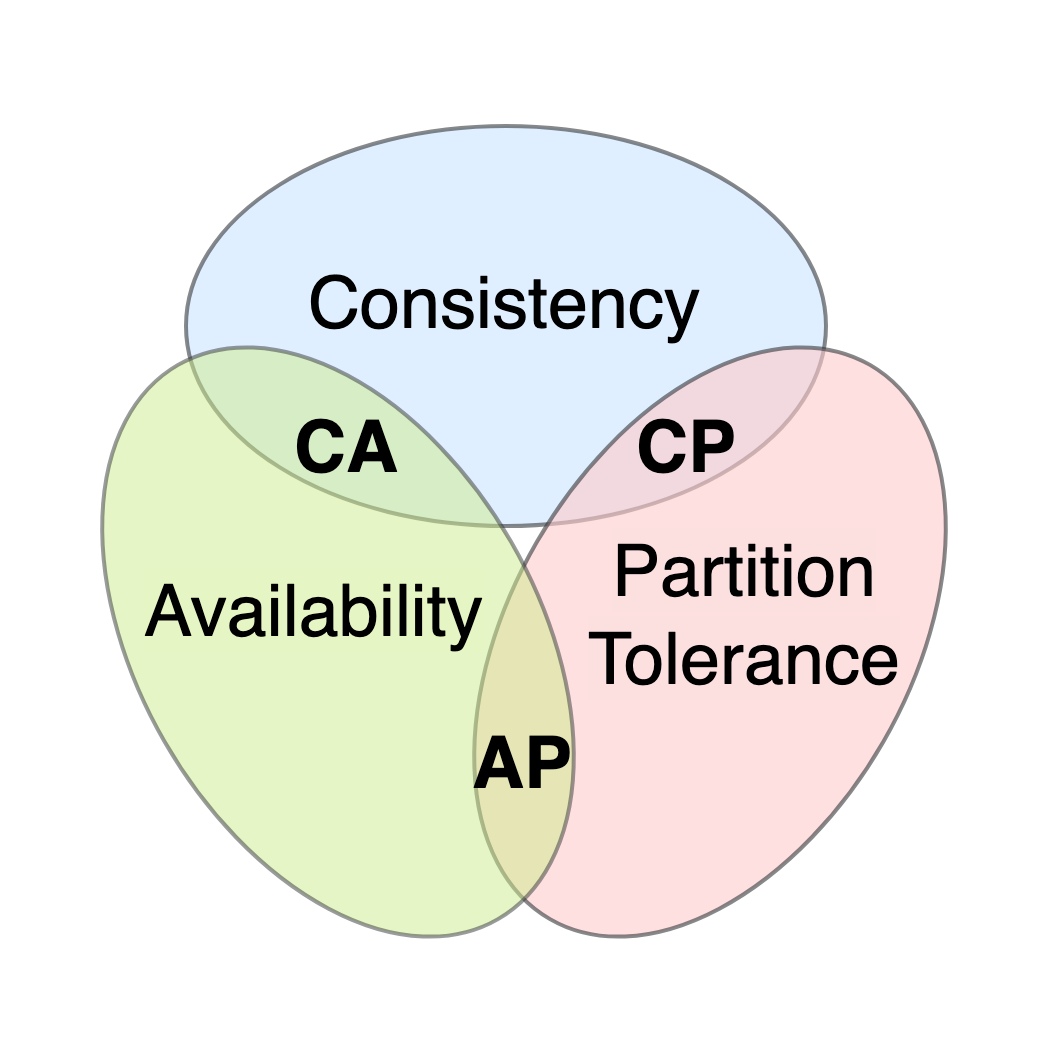
\includegraphics[width=0.5\textwidth]{figuras/CAP_Theorem_Venn_Diagram.png}
    \caption{Diagrama de Venn do Teorema CAP mostrando as interseções entre Consistência, Disponibilidade e Tolerância a Partições.}
    \label{fig:cap_theorem}
\end{figure}

\subsection{Implicações do Teorema CAP em Microserviços}

O Teorema CAP, formulado por Eric Brewer em 2000, afirma que é impossível para um sistema distribuído garantir simultaneamente Consistência (Consistency), Disponibilidade (Availability) e Tolerância à Partição (Partition Tolerance) \cite{brewer2000}. Em outras palavras, em face de uma partição de rede, um sistema deve escolher entre ser consistente ou disponível \cite{brewer2000}. Esse trade-off força os arquitetos de sistemas a priorizar de acordo com os objetivos específicos de sua aplicação.

Na arquitetura de microsserviços, a tolerância à partição é uma necessidade devido à natureza distribuída desses sistemas e à possibilidade de ocorrência de falhas de rede. Isso implica que podem haver momentos em que componentes do sistema não serão capazes de se comunicar. Portanto, os desenvolvedores de microsserviços devem projetar sistemas que possam operar de maneira eficiente mesmo quando partes do sistema estão isoladas umas das outras.

De acordo com Brewer, ao enfrentar uma partição de rede, um sistema deve escolher entre ser consistente ou disponível. Essa escolha depende da natureza e dos requisitos específicos da aplicação \cite{brewer2000}.

\begin{itemize}
    \item \textbf{Consistência:} Priorizar a consistência significa que todos os nós do sistema veem dados idênticos ao mesmo tempo. Isso pode comprometer a disponibilidade, resultando em latências mais altas ou na incapacidade de responder a solicitações durante uma partição de rede. Aplicações que requerem precisão imediata dos dados, como sistemas financeiros, geralmente priorizam a consistência.
    \item \textbf{Disponibilidade:} Priorizar a disponibilidade permite que o sistema continue operando apesar das partições de rede, mas pode resultar em inconsistências temporárias nos dados (consistência eventual). Isso pode ser problemático em sistemas que requerem dados precisos e atualizados em tempo real, mas é aceitável em aplicações onde a alta disponibilidade e performance são mais críticas, como redes sociais ou plataformas de streaming.
\end{itemize}

\subsection{Exemplos Práticos}

\subsubsection{Consistência e Disponibilidade (CA)}

Um sistema que prioriza Consistência e Disponibilidade não pode garantir tolerância a partições. Isso significa que, em caso de falha de rede, o sistema se tornará indisponível até que a comunicação seja restaurada.

\textbf{Exemplo Prático CA:} Em uma aplicação fictícia de reserva de passagens de ônibus, um sistema CA garantiria que todas as reservas são consistentes e disponíveis enquanto não houver falhas de rede. No entanto, se ocorrer uma falha de rede entre servidores, o sistema deve se indisponível para evitar inconsistências. Isso pode ser aceitável em um ambiente onde a consistência imediata dos dados é mais crítica do que a disponibilidade durante falhas de rede.

\subsubsection{Consistência e Tolerância à Partição (CP)}

Um sistema que prioriza Consistência e Tolerância à Partição não pode garantir alta disponibilidade. Isso significa que o sistema pode se tornar indisponível temporariamente para manter a consistência durante falhas de rede.

\textbf{Exemplo Prático CP:} No sistema de reserva de passagens de ônibus, um sistema CP garantiria que as reservas são consistentes mesmo durante falhas de rede. Se os servidores em São Paulo e Rio de Janeiro não puderem se comunicar, o sistema pode bloquear novas reservas temporariamente para evitar inconsistências, garantindo que quando a rede for restaurada, todos os dados estarão em um estado consistente. Isso é crucial em sistemas financeiros ou de reserva onde a precisão dos dados é essencial.

\subsubsection{Disponibilidade e Tolerância à Partição (AP)}

Um sistema que prioriza Disponibilidade e Tolerância à Partição não pode garantir consistência imediata. Isso significa que, em caso de falha de rede, o sistema continuará a operar, mas pode apresentar dados inconsistentes temporariamente.

\textbf{Exemplo Prático AP:} No sistema fictício de reserva de passagens de ônibus, um sistema AP garantiria que os clientes possam fazer reservas mesmo durante falhas de rede. Se os servidores em São Paulo e Rio de Janeiro não puderem se comunicar, ambos os servidores continuarão a aceitar reservas. Isso pode resultar em um estado onde o mesmo assento é reservado para dois clientes diferentes. No entanto, uma vez que a rede seja restaurada, o sistema resolverá essas inconsistências, possivelmente através de um processo de reconciliação. Isso é ideal para sistemas onde a disponibilidade e a capacidade de operação contínua são mais importantes do que a consistência imediata dos dados, como em redes sociais ou portais de notícias.



\chapter{Desafios da Arquitetura de Microsserviços Relacionados à Consistência e Disponibilidade}

Os microsserviços oferecem vantagens significativas, como escalabilidade, flexibilidade e facilidade de manutenção. No entanto, eles também introduzem desafios complexos no gerenciamento de dados. A arquitetura de microsserviços promove a descentralização e a autonomia dos serviços, resultando frequentemente em cada serviço possuir seu próprio banco de dados. Embora essa abordagem seja benéfica para isolar falhas e permitir a independência dos serviços, ela também apresenta várias dificuldades, como problemas de consistência de dados, fragmentação, transações distribuídas e sincronização de dados, entre outros desafios.

\section{Desafios de Consistência de Dados}

Os desafios de consistência de dados em microsserviços estão intimamente relacionados às propriedades ACID, BASE e ao Teorema CAP discutidos anteriormente (ver Seção 2.2.1.2, Seção 2.2.2.3 e Seção 2.3, respectivamente).

\subsection{Fragmentação de Dados}

A fragmentação de dados ocorre quando dados relacionados são armazenados em diferentes bancos de dados geridos por diferentes microsserviços. Cada serviço gerencia seu próprio conjunto de dados, levando a uma fragmentação lógica dos dados que, em uma arquitetura monolítica, seriam normalmente armazenados juntos em um único banco de dados.

Essa fragmentação dificulta a execução de consultas complexas que requerem a agregação de dados de diferentes serviços. Como exemplo, podemos imaginar uma aplicação de comércio eletrônico pode precisar combinar informações de produtos, estoques, pedidos e clientes, que estão distribuídas em diferentes serviços. Orquestrar essas consultas através de múltiplos serviços aumenta a complexidade e a latência, impactando negativamente o desempenho e a eficiência operacional do sistema \cite{fowler2015}.

Além disso, a fragmentação de dados pode levar a problemas de integridade referencial. Em uma aplicação monolítica, a integridade referencial é mantida através de restrições e chaves estrangeiras, geralmente gerenciadas pelo próprio banco de dados ao utilizar um banco relacional. Em um ambiente de microsserviços, não temos esse gerenciamento de forma automatizada. Dessa forma, a manutenção dessas relações deve ser gerenciada pela aplicação, tornando mais difícil e sujeita a erros, aumentando o risco de inconsistências nos dados.

\subsection{Consistência Eventual}

A consistência eventual é um modelo de consistência em sistemas distribuídos onde os dados eventualmente convergem para um estado consistente, desde que não ocorram novas atualizações. Este modelo sacrifica a consistência imediata para melhorar a disponibilidade e a tolerância a falhas.

Nos sistemas distribuídos, a consistência eventual pode resultar em leituras temporariamente inconsistentes, onde diferentes serviços possuem visões divergentes dos dados. Esse comportamento pode ser problemático para operações que exigem uma consistência imediata, como transações financeiras ou reservas de recursos como passagens de ônibus ou quartos em hotéis. Por exemplo, em uma aplicação de reserva de passagens de ônibus, se as atualizações de disponibilidade de assentos não forem propagadas imediatamente para todos os serviços, dois clientes podem acabar reservando o mesmo assento, levando a conflitos e frustrações \cite{vogels2009}.

Além disso, a consistência eventual pode complicar o processo de reconciliação de dados, onde dados inconsistentes precisam ser verificados e sincronizados periodicamente. A reconciliação pode ser um processo complexo e intensivo, exigindo algoritmos sofisticados para resolver conflitos de maneira determinística.

\subsection{Transações Distribuídas}

Gerenciar transações distribuídas em uma arquitetura de microsserviços é um desafio devido à necessidade de garantir as propriedades ACID (Atomicidade, Consistência, Isolamento e Durabilidade) em um ambiente distribuído. Protocolos tradicionais como o Two-Phase Commit (2PC) são frequentemente inadequados devido ao seu impacto negativo na disponibilidade e à possibilidade de bloqueios prolongados \cite{silberschatz2020}.

A coordenação de transações distribuídas pode introduzir latências significativas, impactando negativamente a experiência do usuário. Além disso, a necessidade de garantir a atomicidade das transações em múltiplos serviços pode levar a uma complexidade adicional na implementação e gerenciamento das transações. As falhas em qualquer ponto do processo de transação podem resultar em inconsistências e a necessidade de mecanismos de rollback complexos \cite{gray2006}.

\subsection{Sincronização de Dados entre Serviços}

Garantir a sincronização de dados entre serviços é crucial para manter a consistência e a integridade dos dados em um sistema distribuído. No entanto, a latência de rede, falhas de comunicação e a necessidade de coordenar atualizações em tempo real podem dificultar a manutenção da sincronização.

A latência na propagação de atualizações pode levar a inconsistências temporárias, onde diferentes serviços têm versões diferentes dos mesmos dados. Esse problema é exacerbado em sistemas que requerem alta disponibilidade e baixa latência, onde as atualizações devem ser propagadas rapidamente para evitar inconsistências. Além disso, a sincronização de dados pode ser complicada pela necessidade de garantir a entrega e o processamento ordenado dos eventos de atualização, evitando situações onde eventos mais recentes são processados antes dos mais antigos \cite{pritchett2008}.

\subsection{Conflitos de Escrita e Conciliação}

Conflitos de escrita ocorrem quando múltiplos serviços tentam atualizar o mesmo dado simultaneamente, resultando em versões conflitantes do dado. Resolver esses conflitos é crucial para manter a integridade dos dados em sistemas distribuídos.

Conflitos de escrita podem levar à perda de dados ou inconsistências se não forem resolvidos corretamente. A conciliação dos dados conflitantes pode ser complexa, especialmente quando envolve decisões de negócio. Por exemplo, em uma aplicação de reserva de passagens de ônibus, dois serviços podem tentar reservar o mesmo assento para diferentes clientes simultaneamente. Resolver esse conflito requer uma lógica de negócio clara para determinar qual reserva deve prevalecer e como notificar o cliente cuja reserva foi rejeitada \cite{vogels2009}.

A conciliação de conflitos também pode introduzir latência adicional, impactando a experiência do usuário. Algoritmos de conciliação precisam ser eficientes e eficazes para resolver conflitos rapidamente, minimizando o impacto na operação do sistema. Ferramentas de gerenciamento de dados distribuídos, como Cassandra e Riak, oferecem suporte integrado para técnicas de resolução de conflitos, mas ainda exigem um planejamento cuidadoso e uma implementação robusta \cite{lakshman2010}.

\section{Problemas de Disponibilidade}

\subsection{Falhas de Rede}

As falhas de rede são um dos desafios mais críticos em sistemas de microsserviços. Em um ambiente distribuído, os serviços dependem de uma comunicação constante e confiável entre si. No entanto, a rede pode ser imprevisível e sujeita a falhas. As falhas de rede podem interromper a comunicação entre serviços, resultando em tempo de inatividade e falhas de operação. Isso pode ser particularmente problemático em sistemas que requerem alta disponibilidade e desempenho consistente.

Em um cenário de falha de rede, um serviço pode não conseguir acessar os dados ou serviços necessários para completar uma operação, levando a tempos de espera prolongados e possíveis falhas na execução de transações. Isso pode impactar negativamente a experiência do usuário, especialmente em aplicações críticas onde a disponibilidade contínua é essencial \cite{tanenbaum2007}.

Além disso, as falhas de rede podem levar a problemas de consistência de dados, onde diferentes serviços têm visões divergentes do estado do sistema. A recuperação de falhas de rede exige mecanismos robustos de tolerância a falhas e recuperação automática, o que pode aumentar a complexidade do sistema \cite{brewer2000}.

\subsection{Latência}

A latência é o tempo que leva para uma solicitação de serviço ser processada e uma resposta ser retornada. Em sistemas de microsserviços, a latência pode ser exacerbada pela comunicação entre serviços distribuídos geograficamente e a necessidade de coordenar múltiplas chamadas de serviço para completar uma única operação.

Altos níveis de latência podem impactar negativamente a experiência do usuário, especialmente em aplicações que exigem respostas rápidas e em tempo real. A latência pode ser causada por diversos fatores, incluindo congestionamento de rede, processamento lento de dados, sobrecarga de servidores e ineficiências no código do aplicativo. Reduzir a latência requer otimizações em várias camadas do sistema, incluindo a rede, a infraestrutura de servidores e o próprio software \cite{dean2013}.

\subsection{Isolamento de Falhas}

O isolamento de falhas é uma técnica crítica para garantir que falhas em uma parte do sistema não afetem o restante do sistema. Em um ambiente de microsserviços, onde os serviços são interdependentes, uma falha em um serviço pode potencialmente causar uma cascata de falhas que afeta todo o sistema.

Implementar mecanismos eficazes de isolamento de falhas pode ser desafiador. Isso inclui a utilização de padrões como Circuit Breaker para impedir chamadas repetidas a serviços falhos, Bulkhead para isolar recursos e limitar o impacto de falhas, e Retry para gerenciar tentativas de novas chamadas em caso de falhas temporárias. Além disso, a monitorização contínua e a automação de respostas a falhas são essenciais para detectar e mitigar problemas rapidamente antes que se espalhem \cite{nygard2007}.

\chapter{Padrões de Arquitetura de Microsserviços}

Este capítulo se dedica a explorar em profundidade os padrões de design e arquiteturas fundamentais para o desenvolvimento de sistemas distribuídos robustos e escaláveis, com foco especial em arquiteturas de microsserviços. Este capítulo apresenta uma análise detalhada de quatro padrões essenciais: Command Query Responsibility Segregation (CQRS), Saga, Circuit Breaker e Event Sourcing.

Cada um desses padrões é examinado minuciosamente, explorando suas definições, princípios de funcionamento, vantagens e desvantagens. Além disso, o capítulo fornece exemplos práticos de implementação desses padrões no contexto de uma aplicação fictícia de reserva de passagens, ilustrando como esses conceitos podem ser aplicados em cenários do mundo real. Esta abordagem visa não apenas elucidar os aspectos teóricos desses padrões, mas também demonstrar sua aplicabilidade prática na resolução de desafios comuns em arquiteturas de microsserviços.

\section{Definição de Padrões de Arquitetura}

Padrões de arquitetura são abstrações de soluções de design que resolvem problemas comuns em um contexto específico. Eles não são receitas prontas, mas sim guias que descrevem como estruturar os componentes de um sistema de maneira eficaz. Esses padrões emergem de práticas e experiências acumuladas na indústria e são documentados para serem reutilizados em diferentes projetos \cite{buschmann1996}.

Os padrões de arquitetura fornecem uma visão de alto nível sobre como organizar os componentes de um sistema, estabelecendo diretrizes para a estrutura e a interação desses componentes. Eles ajudam a garantir que os sistemas sejam construídos de maneira consistente, robusta e eficiente. A adoção de padrões de arquitetura pode levar a uma maior previsibilidade no comportamento do sistema, facilitar a comunicação entre equipes de desenvolvimento e melhorar a qualidade geral do software \cite{fowler2011}.

\section{Comparação com Design Patterns}

Enquanto os padrões de arquitetura lidam com a organização macro do sistema, os design patterns (padrões de design) tratam de problemas específicos de implementação em um nível mais granular. Os design patterns são soluções reutilizáveis para problemas comuns encontrados no desenvolvimento de software em nível de código. Eles se concentram em como resolver problemas particulares dentro do contexto da estrutura geral estabelecida pelos padrões de arquitetura \cite{gamma1994}.

Por exemplo, design patterns como Factory, Adapter, e Observer são aplicados para resolver problemas específicos de criação de objetos, estruturação de classes e interação entre objetos. Esses padrões ajudam a melhorar a reutilização, a flexibilidade e a manutenção do código. Em contraste, padrões de arquitetura como Microservices, Layered Architecture, e Event-Driven Architecture fornecem uma visão de alto nível sobre como dividir e organizar o sistema como um todo \cite{fowler2011}.

\section{Importância dos Padrões de Arquitetura em Microsserviços}

Na arquitetura de microsserviços, padrões de arquitetura são fundamentais para abordar os desafios inerentes à construção e operação de sistemas distribuídos. Eles ajudam a enfrentar questões como a comunicação entre serviços, a gestão de transações distribuídas, e a manutenção de consistência e disponibilidade em um ambiente distribuído.

\begin{itemize}
    \item \textbf{Divisão em Serviços:} Um dos princípios fundamentais dos microsserviços é a decomposição de uma aplicação monolítica em serviços menores e independentes. Padrões de arquitetura fornecem diretrizes sobre como realizar essa divisão de forma eficaz, garantindo que cada serviço tenha um escopo bem definido e que a comunicação entre serviços seja eficiente e segura \cite{newman2019}.
    
    \item \textbf{Comunicação entre Serviços:} Em um ambiente de microsserviços, a comunicação entre serviços é uma preocupação central. Padrões como API Gateway e Service Mesh fornecem soluções para gerenciar a comunicação, roteamento, e políticas de segurança entre serviços \cite{richardson2018}.
    
    \item \textbf{Gerenciamento de Dados Distribuídos:} A gestão de dados em um ambiente de microsserviços é complexa devido à necessidade de manter a consistência e a disponibilidade dos dados. Padrões como Event Sourcing e CQRS (Command Query Responsibility Segregation) ajudam a abordar esses desafios, fornecendo métodos para gerenciar estados e transações distribuídas \cite{newman2019}.
\end{itemize}

A seguir, serão descritos os principais padrões de arquitetura utilizados em microsserviços abrangendo suas definições, vantagens, desvantagens e exemplos de implementação com uma aplicação fictícia.

\section{Exemplo de aplicação fictícia}

A ReservaExpress é uma aplicação de reserva de passagens de ônibus que permite aos clientes reservar assentos, consultar a disponibilidade, e gerenciar suas reservas. A aplicação é composta por vários serviços que colaboram para oferecer essas funcionalidades.

A ReservaExpress é uma plataforma de reserva de passagens de ônibus. A aplicação permite que os clientes realizem uma série de operações relacionadas à viagem, incluindo a reserva de assentos, a consulta da disponibilidade de passagens, a visualização de horários de ônibus e a gestão completa de suas reservas.

A aplicação é composta por múltiplos serviços interconectados que trabalham juntos para oferecer um serviço robusto e escalável. Esses serviços incluem o gerenciamento de usuários, a administração de rotas e horários de ônibus, o processamento de pagamentos. Cada serviço é projetado para operar de forma independente, mas interage de maneira harmoniosa para garantir a consistência e a integridade dos dados.

\section{Exemplos de padrões de Arquitetura}
\subsection{CQRS (Command Query Responsibility Segregation)}

\textbf{Definição:} O padrão CQRS (Command Query Responsibility Segregation) é uma abordagem arquitetural que separa as operações de leitura (query) e escrita (command) em sistemas distintos. Greg Young, um dos principais proponentes do CQRS, argumenta que essa separação permite que os sistemas sejam mais escaláveis e mais fáceis de manter \cite{young2010}.

No contexto dos microsserviços, CQRS pode ser implementado criando dois modelos distintos de serviço: um serviço de comando, responsável por manipular dados e executar operações de escrita, e um serviço de consulta, otimizado para operações de leitura. Esses serviços podem usar diferentes bancos de dados e tecnologias para atender melhor suas necessidades específicas.

\begin{figure}[h]
    \centering
    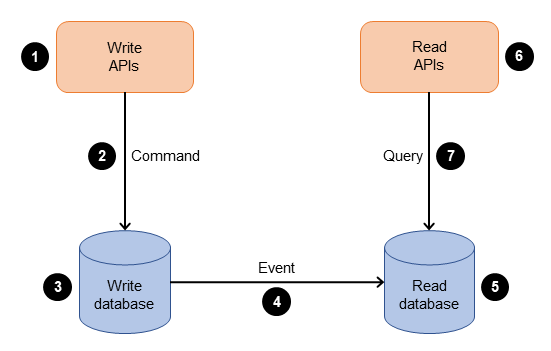
\includegraphics[width=0.8\textwidth]{figuras/cqrs.png}
    \caption{CQRS Pattern}
    \label{fig:cqrs_pattern}
\end{figure}

\textbf{Vantagens:}

\begin{enumerate}
    \item \textbf{Escalabilidade:} A separação das responsabilidades permite que as operações de leitura e escrita sejam escaladas de forma independente. Em sistemas onde as leituras são muito mais frequentes que as escritas, o modelo de leitura pode ser replicado para melhorar a performance sem impactar o modelo de escrita \cite{richardson2018}.
    \item \textbf{Otimização de Performance:} Cada modelo pode ser otimizado para suas operações específicas. O modelo de leitura pode ser altamente denormalizado para otimizar as consultas, enquanto o modelo de escrita pode manter a normalização para garantir a consistência e integridade dos dados \cite{fowler2011}.
    \item \textbf{Manutenção e Evolução do Sistema:} A separação das operações de comando e consulta facilita a manutenção e evolução do sistema. Mudanças nos requisitos de leitura ou escrita podem ser implementadas sem afetar o outro lado, reduzindo o risco de introduzir bugs e facilitando a implementação de novas funcionalidades \cite{young2010}.
    \item \textbf{Consistência e Disponibilidade:} CQRS facilita a implementação de consistência eventual em sistemas distribuídos. As operações de escrita podem ser propagadas para o modelo de leitura de forma assíncrona, permitindo que o sistema continue disponível mesmo durante a atualização de dados \cite{richardson2018}.
\end{enumerate}

\textbf{Desvantagens:}

\begin{enumerate}
    \item \textbf{Complexidade:} A implementação de CQRS pode aumentar a complexidade do sistema. Manter dois modelos separados requer um esforço adicional de desenvolvimento e manutenção, além de aumentar a complexidade da infraestrutura necessária para suportar ambos os modelos \cite{fowler2011}.
    \item \textbf{Gerenciamento de Eventos:} CQRS geralmente é implementado em conjunto com o padrão Event Sourcing, o que introduz a necessidade de gerenciar eventos de forma eficiente. A consistência eventual pode ser complexa de implementar corretamente, exigindo um mecanismo robusto de processamento e armazenamento de eventos \cite{young2010}.
    \item \textbf{Latência de Consistência:} A propagação assíncrona das operações de escrita para o modelo de leitura pode introduzir latência na consistência dos dados. Isso significa que, após uma operação de escrita, pode haver um atraso até que o modelo de leitura seja atualizado, resultando em leituras temporariamente inconsistentes \cite{richardson2018}.
\end{enumerate}

\subsubsection{Exemplo de implementação na aplicação fictícia}

\textbf{Componentes:}

\begin{itemize}
    \item \textbf{Serviço de Comando:}
    \begin{itemize}
        \item \textbf{Responsabilidades:} Processa todas as operações de escrita, como reservar um assento, cancelar uma reserva ou atualizar os detalhes de uma viagem.
        \item \textbf{Banco de Dados:} Utiliza um banco de dados relacional (por exemplo, PostgreSQL) para garantir consistência e integridade dos dados.
        \item \textbf{Fluxo de Trabalho:} Quando um cliente faz uma reserva, o serviço valida a solicitação e grava os dados no banco de dados. Em seguida, emite um evento "ReservaCriada".
    \end{itemize}

    \item \textbf{Serviço de Consulta:}
    \begin{itemize}
        \item \textbf{Responsabilidades:} Otimizado para operações de leitura, como verificar a disponibilidade de assentos, visualizar reservas existentes e consultar horários de viagens.
        \item \textbf{Banco de Dados:} Utiliza um banco de dados NoSQL (por exemplo, MongoDB) para consultas rápidas e escaláveis, com um modelo de dados denormalizado para otimizar o desempenho das consultas.
        \item \textbf{Fluxo de Trabalho:} Recebe eventos do Serviço de Comando e atualiza seu modelo de leitura de forma assíncrona para refletir as mudanças no sistema.
    \end{itemize}
\end{itemize}

\textbf{Exemplo de Fluxo:}

\begin{enumerate}
    \item O cliente faz uma solicitação de reserva.
    \item O Serviço de Comando processa a solicitação, verifica a disponibilidade do assento, e grava a reserva no banco de dados.
    \item O Serviço de Comando emite um evento "ReservaCriada".
    \item O Serviço de Consulta recebe o evento "ReservaCriada" e atualiza seu banco de dados NoSQL para refletir a nova reserva.
\end{enumerate}

\subsection{Saga}

\textbf{Definição:} O padrão Saga é uma abordagem para gerenciar transações distribuídas em sistemas de microsserviços, garantindo a consistência de dados em ambientes onde transações ACID tradicionais não são viáveis. Uma Saga é uma sequência de transações que atualizam diferentes serviços. Se uma transação falhar, a Saga executa uma série de passos de compensação para desfazer as alterações feitas pelas transações anteriores. Uma Saga é uma longa atividade que pode ser dividida em um conjunto de transações menores e independentes, cada uma das quais pode ser compensada caso ocorra uma falha \cite{garcia-molina1987}.

No contexto dos microsserviços, uma Saga permite que uma transação que abrange múltiplos serviços seja dividida em várias transações locais, cada uma das quais pode ser revertida de forma independente se necessário. Isso ajuda a manter a consistência dos dados sem a necessidade de uma transação global.

\textbf{Vantagens:}

\begin{enumerate}
    \item \textbf{Consistência em Sistemas Distribuídos:} Sagas permitem que sistemas de microsserviços mantenham a consistência de dados sem precisar de uma transação global. Cada serviço pode aplicar suas alterações de maneira independente e, em caso de falha, realizar compensações para reverter as mudanças \cite{richardson2018}.
    \item \textbf{Escalabilidade e Desempenho:} Por não depender de bloqueios e coordenação centralizada, Sagas melhoram a escalabilidade e o desempenho do sistema. Transações locais são mais rápidas e menos propensas a criar gargalos \cite{fowler2011}.
    \item \textbf{Resiliência:} A capacidade de compensar transações falhadas aumenta a resiliência do sistema. Mesmo se uma parte da transação falhar, o sistema pode continuar a operar e recuperar-se das falhas aplicando as compensações necessárias \cite{garcia-molina1987}.
\end{enumerate}

\textbf{Desvantagens:}

\begin{enumerate}
    \item \textbf{Complexidade:} Implementar Sagas pode ser complexo, especialmente ao definir e gerenciar as operações de compensação. Cada transação deve ter uma transação compensatória associada, o que aumenta o esforço de desenvolvimento \cite{richardson2018}.
    \item \textbf{Latência:} A execução de passos de compensação pode introduzir latência adicional, especialmente se várias transações precisam ser revertidas. Isso pode impactar a experiência do usuário em casos de falhas frequentes \cite{fowler2011}.
    \item \textbf{Consistência Eventual:} Sagas garantem consistência eventual, o que significa que, temporariamente, os dados podem estar inconsistentes enquanto as compensações são aplicadas. Isso pode ser aceitável para algumas aplicações, mas problemático para outras \cite{garcia-molina1987}.
\end{enumerate}

\textbf{Exemplo de Implementação}

\textbf{Coordenação e Compensação:} Em um sistema de microsserviços, a coordenação das transações distribuídas por meio de Sagas envolve definir claramente os passos da transação e suas respectivas operações de compensação. A lógica de coordenação pode ser implementada de duas formas principais:

\begin{enumerate}
    \item \textbf{Orquestração Centralizada:} Um serviço central coordena a execução de cada passo da Saga. Esse orquestrador inicia cada transação local e, em caso de falha, chama as operações de compensação necessárias. Esse método é mais simples de implementar, pois a lógica de coordenação está concentrada em um único serviço.
    \item \textbf{Coreografia Descentralizada:} Cada serviço participante é responsável por iniciar a próxima etapa da Saga ao completar sua transação local. Se uma falha ocorrer, cada serviço participante é responsável por executar suas operações de compensação. Esse método elimina o ponto único de falha do orquestrador, mas aumenta a complexidade da implementação.
\end{enumerate}

\subsubsection{Exemplo de implementação na aplicação fictícia}

\textbf{Componentes:}

\begin{itemize}
    \item \textbf{Serviço de Reserva:}
    \begin{itemize}
        \item \textbf{Responsabilidades:} Verifica a disponibilidade de assentos e confirma as reservas.
        \item \textbf{Operações de Compensação:} Cancela a reserva e libera o assento se a transação falhar.
    \end{itemize}

    \item \textbf{Serviço de Pagamento:}
    \begin{itemize}
        \item \textbf{Responsabilidades:} Processa os pagamentos dos clientes.
        \item \textbf{Operações de Compensação:} Reembolsa o valor ao cliente se a transação falhar.
    \end{itemize}
\end{itemize}

\textbf{Exemplo de Fluxo:}

\begin{enumerate}
    \item O cliente solicita uma reserva.
    \item O Serviço de Reserva verifica a disponibilidade do assento.
    \item O Serviço de Pagamento processa o pagamento.
    \item Se o pagamento for bem-sucedido, o Serviço de Reserva confirma a reserva.
    \item Se qualquer etapa falhar, as operações de compensação são executadas:
    \begin{itemize}
        \item Se a verificação de disponibilidade falhar, a Saga termina sem ação.
        \item Se o pagamento falhar, o valor é reembolsado.
        \item Se a confirmação da reserva falhar, o pagamento é reembolsado e o assento é liberado.
    \end{itemize}
\end{enumerate}

\subsection{Circuit Breaker}

\textbf{Definição:} O padrão Circuit Breaker é uma abordagem de design utilizada para aumentar a resiliência de sistemas distribuídos, protegendo serviços contra falhas em cascata e melhorando a tolerância a falhas. Martin Fowler descreve o Circuit Breaker como um dispositivo que impede o sistema de fazer chamadas repetidas a um componente que está falhando, evitando assim sobrecarregar e potencialmente degradar o desempenho de outros componentes \cite{fowler2014}.

O Circuit Breaker possui três estados principais:

\begin{enumerate}
    \item \textbf{Fechado (Closed):} As chamadas são permitidas e os erros são monitorados.
    \item \textbf{Aberto (Open):} As chamadas são bloqueadas por um período de tempo após um número predeterminado de falhas.
    \item \textbf{Meio-Aberto (Half-Open):} Algumas chamadas são permitidas para testar se o serviço falho se recuperou.

\end{enumerate}
{Operação do Circuit Breaker:} O Circuit Breaker monitora as chamadas entre serviços e conta o número de falhas dentro de um período específico. Se o número de falhas exceder um limite predeterminado, o Circuit Breaker abre, bloqueando novas tentativas de chamada ao serviço problemático por um período definido (timeout). Após o timeout, o Circuit Breaker entra em estado Meio-Aberto, permitindo algumas chamadas para verificar se o serviço se recuperou. Se as chamadas forem bem-sucedidas, o Circuit Breaker volta ao estado Fechado; caso contrário, retorna ao estado Aberto.

\textbf{Vantagens:}

\begin{enumerate}
    \item \textbf{Prevenção de Falhas em Cascata:} O Circuit Breaker impede que falhas em um serviço propaguem-se para outros serviços, protegendo o sistema contra falhas em cascata que podem levar a uma degradação geral do sistema \cite{fowler2014}.
    \item \textbf{Melhoria da Resiliência:} Ao isolar serviços falhos, o Circuit Breaker aumenta a resiliência do sistema, permitindo que outros serviços continuem a operar normalmente enquanto o serviço problemático se recupera \cite{nygard2007}.
    \item \textbf{Redução de Latência:} O Circuit Breaker evita que chamadas repetidas a serviços falhos causem latência desnecessária, melhorando a responsividade geral do sistema \cite{nygard2007}.
\end{enumerate}

\textbf{Desvantagens:}

\begin{enumerate}
    \item \textbf{Complexidade Adicional:} Implementar o Circuit Breaker adiciona complexidade ao sistema, exigindo monitoramento e gerenciamento cuidadoso dos estados do Circuit Breaker \cite{fowler2014}.
    \item \textbf{Latência na Recuperação:} Durante o período em que o Circuit Breaker está aberto, novas tentativas de chamadas são bloqueadas, o que pode introduzir latência na recuperação do serviço caso ele se recupere rapidamente \cite{nygard2007}.
    \item \textbf{Possibilidade de Falsos Positivos:} Se mal configurado, o Circuit Breaker pode ativar-se erroneamente, bloqueando chamadas para serviços que estão operando normalmente, o que pode impactar negativamente a disponibilidade do sistema \cite{nygard2007}.
\end{enumerate}

\subsubsection{Exemplo de implementação na aplicação fictícia}

\textbf{Componentes:}

\begin{itemize}
    \item \textbf{Serviço de Reserva:}
    \begin{itemize}
        \item \textbf{Responsabilidades:} Gerencia a disponibilidade e confirmação de reservas.
    \end{itemize}

    \item \textbf{Serviço de Pagamento:}
    \begin{itemize}
        \item \textbf{Responsabilidades:} Processa pagamentos das reservas.
    \end{itemize}
\end{itemize}

\textbf{Exemplo de Fluxo:}

\begin{enumerate}
    \item O Serviço de Reserva faz chamadas ao Serviço de Pagamento para processar pagamentos.
    \item O Circuit Breaker monitora essas chamadas.
    \item Se o Serviço de Pagamento falhar repetidamente, o Circuit Breaker abre, bloqueando novas tentativas de pagamento.
    \item Durante o período em que o Circuit Breaker está aberto, o Serviço de Reserva retorna respostas rápidas ao cliente, informando sobre a indisponibilidade temporária do serviço de pagamento.
    \item Após um timeout, o Circuit Breaker entra em estado Meio-Aberto, permitindo algumas chamadas de teste.
    \item Se as chamadas de teste forem bem-sucedidas, o Circuit Breaker fecha novamente; se falharem, ele reabre.
\end{enumerate}

\subsection{Event Sourcing}

\textbf{Definição:}

No padrão Event Sourcing, cada mudança de estado em um sistema é capturada como um evento. Esses eventos são armazenados em um repositório de eventos e podem ser reproduzidos a qualquer momento para reconstruir o estado do sistema. Event Sourcing é um padrão onde as mudanças de estado de um objeto são armazenadas como uma sequência de eventos, e o estado atual do objeto é derivado desses eventos \cite{fowler2005}.

\textbf{Vantagens:}

\begin{enumerate}
    \item \textbf{Auditabilidade e Histórico Completo:} Event Sourcing permite que todo o histórico de mudanças do sistema seja armazenado. Isso é particularmente útil para auditoria e conformidade, pois cada alteração pode ser rastreada até sua origem \cite{fowler2005}.
    \item \textbf{Consistência e Reprodutibilidade:} Como o estado do sistema pode ser reconstruído a partir de eventos, é fácil garantir a consistência do estado em diferentes nós de um sistema distribuído. Eventos são imutáveis e podem ser reproduzidos para sincronizar estados \cite{richardson2018}.
    \item \textbf{Escalabilidade:} Event Sourcing facilita a escalabilidade, pois os eventos podem ser distribuídos e processados de maneira assíncrona. Serviços diferentes podem reagir a eventos específicos, permitindo um processamento paralelo e distribuído \cite{vernon2013}.
    \item \textbf{Flexibilidade na Recuperação de Estado:} Permite reverter o estado do sistema para qualquer ponto no tempo, simplesmente reproduzindo os eventos até aquele momento. Isso é útil para depuração e recuperação de falhas \cite{fowler2005}.
\end{enumerate}

\textbf{Desvantagens:}

\begin{enumerate}
    \item \textbf{Complexidade:} Implementar Event Sourcing adiciona complexidade ao sistema. A lógica para gerenciar e reproduzir eventos, além de garantir a integridade e a ordem dos eventos, pode ser difícil de implementar corretamente \cite{richardson2018}.
    \item \textbf{Consistência Eventual:} Como os eventos são processados de maneira assíncrona, pode haver um atraso até que todos os serviços estejam sincronizados com o estado mais recente. Isso pode resultar em uma consistência eventual dos dados \cite{vernon2013}.
    \item \textbf{Crescimento do Repositório de Eventos:} O armazenamento de todos os eventos pode levar a um crescimento significativo do repositório de eventos ao longo do tempo. Gerenciar e arquivar eventos antigos pode ser necessário para manter a performance e a capacidade de armazenamento \cite{fowler2005}.
\end{enumerate}

\subsubsection{Exemplo de implementação na aplicação fictícia}

\textbf{Componentes:}

\begin{itemize}
    \item \textbf{Repositório de Eventos:}
    \begin{itemize}
        \item \textbf{Responsabilidades:} Armazena todos os eventos que representam mudanças de estado no sistema.
    \end{itemize}

    \item \textbf{Serviços de Processamento de Eventos:}
    \begin{itemize}
        \item \textbf{Responsabilidades:} Geram eventos ao processar mudanças de estado e aplicam esses eventos para atualizar o estado do sistema.
    \end{itemize}
\end{itemize}

\textbf{Exemplo de Fluxo:}

\begin{enumerate}
    \item O cliente reserva um assento.
    \item Um evento "AssentoReservado" é gerado e armazenado no repositório de eventos.
    \item Se a reserva for cancelada, um evento "ReservaCancelada" é gerado e armazenado.
    \item Para determinar a disponibilidade atual dos assentos, o sistema reproduz todos os eventos "AssentoReservado" e "ReservaCancelada" na ordem em que ocorreram.
\end{enumerate}

\chapter{Ferramentas e Frameworks que Ajudam na Implementação de Padrões de Microsserviço em Bancos de Dados}

Este capítulo apresenta uma análise abrangente das ferramentas e frameworks mais relevantes para a implementação de padrões de microsserviços em sistemas de banco de dados. Este capítulo explora uma variedade de soluções tecnológicas, incluindo Helidon, Spring Cloud, Eclipse Vert.x, Lagom, Akka, Eventuate e Axon Framework. Cada uma dessas ferramentas é examinada em detalhe, destacando suas funcionalidades principais, características distintivas e aplicabilidade na construção de arquiteturas de microsserviços robustas e escaláveis. Através desta análise, o capítulo busca fornecer uma visão prática e comparativa das opções disponíveis para desenvolvedores e arquitetos de sistemas, auxiliando na escolha das ferramentas mais adequadas para diferentes cenários de implementação de microsserviços.

\section{Helidon}
Helidon é uma coleção de bibliotecas Java para construir microsserviços. Desenvolvido pela Oracle, Helidon oferece duas variantes principais: Helidon SE e Helidon MP. Helidon SE é uma biblioteca leve e funcional, enquanto Helidon MP é compatível com as especificações MicroProfile, facilitando a criação de microsserviços baseados em padrões Java EE.

\subsection{Funcionalidades e Características}
\begin{itemize}
    \item \textbf{MicroProfile Support}: Helidon MP oferece suporte completo às especificações MicroProfile, permitindo a criação de microsserviços com padrões conhecidos da indústria \cite{Helidon2021}.
    \item \textbf{Leve e Modular}: Helidon SE é projetado para ser leve e modular, oferecendo uma base mínima para a construção de microsserviços altamente eficientes \cite{Helidon2021}.
    \item \textbf{Reatividade}: Helidon suporta programação reativa, proporcionando alta performance e baixa latência \cite{Helidon2021}.
\end{itemize}

Mais detalhes podem ser encontrados em: \url{https://helidon.io}.


\section{Spring Cloud}
Spring Cloud é um conjunto de ferramentas projetado para ajudar os desenvolvedores a construir sistemas distribuídos baseados em microsserviços. Ele oferece uma ampla gama de funcionalidades para configuração, descoberta de serviços, roteamento, gerenciamento de circuit breakers e muito mais.

\subsection{Funcionalidades e Características}
\begin{itemize}
    \item \textbf{Configuração Distribuída}: Spring Cloud Config Server permite gerenciar configurações de forma centralizada para todos os microsserviços \cite{SpringCloud2021}.
    \item \textbf{Descoberta de Serviços}: Utiliza Eureka para registro e descoberta de serviços, facilitando a comunicação entre microsserviços \cite{SpringCloud2021}.
    \item \textbf{Circuit Breaker}: Integração com Resilience4j para implementar circuit breakers, garantindo resiliência no sistema \cite{SpringCloud2021}.
    \item \textbf{Roteamento Inteligente}: Utiliza Zuul ou Spring Cloud Gateway para roteamento de requisições entre microsserviços \cite{SpringCloud2021}.
\end{itemize}

Mais detalhes podem ser encontrados em: \url{https://spring.io/projects/spring-cloud}.


\section{Eclipse Vert.x}
Eclipse Vert.x é uma toolkit para a construção de aplicações reativas e poliglota sobre a JVM. Ele permite a criação de microsserviços assíncronos e reativos, suportando vários padrões de design como CQRS e Event Sourcing.

\subsection{Funcionalidades e Características}
\begin{itemize}
    \item \textbf{Reatividade}: Suporte completo para programação reativa, oferecendo alta performance e escalabilidade \cite{Vertx2021}.
    \item \textbf{Poliglota}: Suporte para múltiplas linguagens de programação, incluindo Java, Kotlin, JavaScript, e Groovy \cite{Vertx2021}.
    \item \textbf{Modular}: Arquitetura modular que permite adicionar funcionalidades conforme necessário \cite{Vertx2021}.
    \item \textbf{Clusterização}: Suporte nativo para clusterização, permitindo a distribuição de microsserviços em múltiplos nós \cite{Vertx2021}.
\end{itemize}

Mais detalhes podem ser encontrados em:  \url{https://vertx.io}.


\section{Lagom}
Lagom, desenvolvido pela Lightbend, é um framework open-source para a construção de sistemas de microsserviços com suporte nativo para CQRS e Event Sourcing. Ele é projetado para facilitar a criação de microsserviços escaláveis e resilientes.

\subsection{Funcionalidades e Características}
\begin{itemize}
    \item \textbf{CQRS e Event Sourcing}: Suporte nativo para a separação de comandos e consultas, bem como a persistência de eventos \cite{Lagom2021}.
    \item \textbf{Integração com Akka}: Utiliza Akka para comunicação entre serviços, proporcionando alta performance e baixa latência \cite{Boner2014}.
    \item \textbf{Escalabilidade}: Projetado para sistemas distribuídos, facilitando a criação de serviços independentes que podem ser escalados conforme necessário \cite{Lagom2021}.
\end{itemize}

Mais detalhes podem ser encontrados em: \url{https://www.lagomframework.com}.


\section{Akka}
Akka, também desenvolvido pela Lightbend, é uma toolkit para construção de aplicações concorrentes, distribuídas e resilientes. Ele oferece uma base robusta para a criação de microsserviços, especialmente aqueles que requerem alta escalabilidade e resiliência.

\subsection{Funcionalidades e Características}
\begin{itemize}
    \item \textbf{Modelo de Atores}: Utiliza o modelo de atores para facilitar a construção de sistemas concorrentes e distribuídos \cite{Akka2021}.
    \item \textbf{Resiliência}: Suporte robusto para construção de sistemas resilientes com supervisão e gerenciamento de falhas \cite{Akka2021}.
    \item \textbf{Clusterização}: Suporte nativo para clusterização, permitindo a distribuição de atores em múltiplos nós \cite{Akka2021}.
    \item \textbf{Streams Reativos}: Suporte para streams reativos, permitindo processamento de dados em tempo real \cite{Akka2021}.
\end{itemize}

Mais detalhes podem ser encontrados em: \url{https://akka.io}.


\section{Eventuate}
Eventuate é uma plataforma open-source que oferece suporte a Event Sourcing e CQRS para aplicações baseadas em microsserviços. Ela facilita a construção de sistemas resilientes e escaláveis através da persistência de eventos.

\subsection{Funcionalidades e Características}
\begin{itemize}
    \item \textbf{Event Sourcing}: Armazenamento e recuperação de eventos para facilitar a implementação de Event Sourcing \cite{Eventuate2021}.
    \item \textbf{CQRS}: Suporte para a separação de comandos e consultas, facilitando a escalabilidade e a manutenção do sistema \cite{richardson2018}.
    \item \textbf{Consistência Eventual}: Suporte a consistência eventual, garantindo que os dados eventualmente converjam para um estado consistente em sistemas distribuídos \cite{helland2015}.
\end{itemize}

Mais detalhes podem ser encontrados em: \url{http://eventuate.io}.


\section{Axon Framework}
O Axon Framework é uma das ferramentas mais robustas e amplamente utilizadas para a implementação de CQRS e Event Sourcing em aplicações Java. Desenvolvido para facilitar a criação de sistemas escaláveis e flexíveis, o Axon fornece uma infraestrutura completa para o gerenciamento de comandos, eventos e sagas \cite{AxonIQ2021}.

\subsection{Funcionalidades e Características}
\begin{itemize}
    \item \textbf{CQRS}: Axon oferece suporte completo para a separação de comandos e consultas, facilitando a escalabilidade e a manutenção do sistema \cite{richardson2018}.
    \item \textbf{Event Sourcing}: O framework suporta a persistência de eventos e oferece ferramentas para gerenciar a armazenagem e recuperação de eventos \cite{fowler2005}.
    \item \textbf{Sagas}: Axon facilita a coordenação de transações distribuídas através do padrão Saga, permitindo que cada transação local possa ser compensada em caso de falha \cite{garcia-molina1987}.
    \item \textbf{Integração com Spring}: Axon se integra perfeitamente com o Spring Framework, permitindo que desenvolvedores utilizem as funcionalidades do Spring Boot para configuração e gerenciamento de dependências \cite{AxonIQ2021}.
    \item \textbf{Escalabilidade}: Projetado para suportar sistemas distribuídos e escaláveis, permitindo a implementação de microsserviços que podem ser desenvolvidos, testados e implantados de forma independente \cite{richardson2018}.
\end{itemize} 

Mais detalhes podem ser encontrados em: \url{https://axoniq.io}.

\chapter{Considerações Finais}

Este capítulo propõe a implementação prática dos padrões de arquitetura de microsserviços discutidos anteriormente, utilizando a aplicação fictícia "ReservaExpress" introduzida no Capítulo 4.4. A construção deste estudo de caso visa aplicar e avaliar diversos padrões de arquitetura de microsserviços, proporcionando uma análise detalhada de seu impacto em um cenário de aplicação real.

\section{Objetivos do Estudo de Caso}

O desenvolvimento da aplicação "ReservaExpress" tem como objetivos principais:

\begin{enumerate}
    \item Implementar um sistema de software funcional que incorpore os padrões de arquitetura de microsserviços.
    \item Avaliar a eficácia desses padrões na melhoria da consistência e disponibilidade da aplicação, conforme o teorema CAP.
    \item Documentar as lições aprendidas e os desafios enfrentados durante a implementação, fornecendo um guia prático para futuras implementações e pesquisas.
\end{enumerate}

\section{Metodologia e Cronograma Propostos}

A metodologia para o desenvolvimento e avaliação da "ReservaExpress" abrange as seguintes fases, alinhadas com o cronograma de execução:

\begin{enumerate}
    \item \textbf{Estudo e Preparação:} Aprofundamento no estudo das tecnologias relevantes e seleção das ferramentas e frameworks adequados para o desenvolvimento.
    
    \item \textbf{Design e Planejamento:} Elaboração da arquitetura da aplicação e definição dos casos de uso e cenários de teste.
    
    \item \textbf{Implementação:} Desenvolvimento dos microsserviços conforme os padrões selecionados, com implementação iterativa, incorporando feedback e ajustes.
    
    \item \textbf{Testes e Validação:} Execução de testes unitários, de integração e de carga, além da avaliação da performance e escalabilidade da aplicação.
    
    \item \textbf{Documentação e Finalização:} Documentação do processo de desenvolvimento e resultados, análise final, elaboração das conclusões, e revisão e refinamento do texto do TCC.
\end{enumerate}

O cronograma proposto é flexível e pode ser ajustado conforme o progresso do projeto e eventuais desafios encontrados durante o desenvolvimento. A tabela a seguir apresenta uma visão geral do cronograma:

\begin{table}[h]
    \centering
    \begin{tabular}{|p{4cm}|p{8cm}|}
        \hline
        \textbf{Período} & \textbf{Atividade} \\
        \hline
        Semanas 1-4 & Estudo e Preparação \\
        \hline
        Semanas 5-8 & Design e Planejamento \\
        \hline
        Semanas 9-16 & Implementação \\
        \hline
        Semanas 17-20 & Testes e Validação \\
        \hline
        Semanas 21-24 & Documentação e Finalização \\
        \hline
    \end{tabular}
    \caption{Cronograma do Estudo de Caso "ReservaExpress"}
    \label{tab:cronograma}
\end{table}

Este cronograma fornece uma estrutura geral para o desenvolvimento do projeto, permitindo flexibilidade na execução e ajustes conforme necessário ao longo do processo.

% \lipsum[1-5]



% \chapter{Algumas notas sobre bibliografia}


% \par O arquivo \textit{referencias.bib} é o nome padrão das referências para este modelo. Para alterá-lo modifique o argumento entre chaves na definição de bibliografia.


%    \section{Modelos de citação}
%       \par No arquivo modelo de referências, também existem alguns exemplos de diferentes classes de citações. Todas elas podem ser usadas com o \textit{$\backslash$cite$\{$label$\}$} ou \textit{$\backslash$citeonline$\{$label$\}$}, dependendo da forma de citação\footnote{Este é um teste de nota de rodapé}.

% 	\par Além disso, pode-se incluir obras na bibliografia que nortearam o trabalho mesmo que elas não apareçam diretamente no texto, utilizando o comando \textit{$\backslash$nocite$\{$label$\}$}. Além disso, pode-se citar vários trabalhos em conjunto, por exemplo:
	
% 	\begin{center}\rule{0.5\textwidth}{1pt}\\$\backslash cite\{label1,label2,label3,...\}$\end{center}

% 	\begin{verbatim}
% 	Os ventos do norte não movem moinhos \cite{tcc:mintegui2014, 
% 	diss:anabor2004, tese:anabor2008, livro:halliday28ed, 
% 	livro:fedorova:v1, site:amsglo:fog}.
% 	\end{verbatim}
	    
% 	\par Os ventos do norte\footnote{Este é um teste de nota de rodapé} não movem moinhos \cite{tcc:mintegui2014,diss:anabor2004,tese:anabor2008,livro:halliday28ed,livro:fedorova:v1,site:amsglo:fog}.
        
%         \begin{center}\rule{0.5\textwidth}{1pt}\\$\backslash citeonline\{label1,label2,label3,...\}$\end{center}
        
% 	\begin{verbatim}
% 	Segundo \citeonline{cap:livro:djuric1994, livro:aris1989, 
% 	livro:cotton1989, cap:livro:wyngaard1981, livro:fedorova:v1, 
% 	artigo:fujita1981,puhalesBLT2010,artigo:janjic2002,
% 	cbmet:anabor2012,site:wrfhome}, os ventos do norte não movem moinhos.
% 	\end{verbatim}
            
%         \par Segundo \citeonline{cap:livro:djuric1994, livro:aris1989, livro:cotton1989, cap:livro:wyngaard1981, livro:fedorova:v1, artigo:fujita1981,puhalesBLT2010,artigo:janjic2002,cbmet:anabor2012,site:wrfhome}, os ventos\footnote{Este é um teste de nota de rodapé} do norte não movem moinhos.
%         \begin{center}\rule{0.5\textwidth}{1pt}\end{center}   
%          \par OBS: Trabalhos com mais de três autores aparecerão com a abreviatura ``et al'' no corpo do texto, porém todos os nomes da bibliografia (norma da UFSM que é definida nas opões do abntcite nas definições do arquivo). 
  
%   \subsection{O comando \textit{apud}}

%   \par A citação \textit{apud} ocorre quando você cita algum autor através de outra obra, sem ter consultado-a propriamente. Neste caso a citação é feita da seguinte forma:
%   \begin{center}
%   \rule{0.5\textwidth}{1pt}\\
%   $\backslash apud\{material\_citado\_no\_material\_lido\}\{material\_lido\}$ \\
%   \end{center}
% \begin{verbatim}
% Sobre a circulação geral da atmosfera pode-se dizer que os ventos do norte
% não movem moinhos \apud{apud:richardson1922}{livro:monin:v1}.
% \end{verbatim}
  
%   Sobre a circulação geral da atmosfera pode-se dizer que os ventos do nortenão movem moinhos \apud{apud:richardson1922}{livro:monin:v1}.
% \begin{center}\rule{0.5\textwidth}{1pt}\end{center}  
%   \par Nesse caso, na bibliografia só constará a obra consultada e não aquele referenciada pela obra. Para que isso ocorra naturalmente, a obra consultada deve ser incluída normalmente no arquivo referencias.bib enquanto a obra referenciada indiretamente deve ser incluída com a opção \textit{@hidden}, conforme o modelo de referências\footnote{Isto é um teste de nota de rodapé}.

%       \subsubsection{\textit{Apud on line}}

      
%       \par O \textit{apudonline} se aplica da mesma maneira que o \textit{apud} descrito anteriormente. O termo \textit{on line} é alusivo ao \textit{$\backslash$citeonline$\{$label$\}$} definido no abntex. Nesse caso a citação é feita da seguinte forma:
%       \begin{center}
%       \rule{0.5\textwidth}{1pt}
%             $\backslash apudonline\{material\_citado\_no\_material\_lido\}\{material\_lido\}$ \\
% 	    \end{center}

%  \begin{verbatim}
% Segundo \apudonline{apud:richardson1922}{livro:monin:v1}, os ventos do
% norte não movem moinhos.
% \end{verbatim}

%             Segundo \apudonline{apud:richardson1922}{livro:monin:v1}, os ventos do norte não movem moinhos.

% \subsubsection{Citação longa}
	
% 	\begin{quoting}[rightmargin=0cm,leftmargin=4cm]
% 		\begin{singlespace}
% 			{\footnotesize
% 				\noindent Texto da citação sem ser identado e com recuo de 4cm, fonte tamanho 10 e espaçamento simples.  \lipsum[2] Termine com ponto antes da citação.  \cite{man:MDTUFSM2015}.
% 			}
% 		\end{singlespace}
% 	\end{quoting}

%        \paragraph{Teste de seção quinária}
       
%        \par Texto texto texto.
       
       
%          \chapter{Tabelas, figuras, quadros, ilustrações e gráficos}
         
%          \par Na MDT da UFSM há uma clara diferença entre tabelas e quadros, quanto a sua apresentação. Aqui, para inserir tabelas usa-se o ambiente tradicionalmente definido \textit{table}. A partir deste modelo simples:
        
%          \begin{verbatim}
% 		\begin{table}[ht]
% 		\centering
% 		\caption{Modelo de tabela para MDT-UFSM.}
% 		\begin{tabular}{ c c c }
% 		\hline
% 		Abacate & Banana & Canela \\
% 		\hline
% 		21 & 34 & 56 \\
% 		-3 & 245 & 23 \\
% 		-25 & -0,57 & 2 \\
%                 \hline
%                  \end{tabular}
% 		\fonte{Adaptado de \citeonline{livro:halliday28ed}.}
% 		\end{table}
% 	  \end{verbatim}
         
%          \noindent resulta:
         
%          \begin{table}[ht]
%          \centering
%          \caption{Modelo de tabela para MDT-UFSM.}
%          \begin{tabular}{ c c c }
%          \hline
%          Abacate & Banana & Canela \\
%          \hline
%          21 & 34 & 56 \\
%          -3 & 245 & 23 \\
%          -25 & -0,57 & 2 \\
%          \hline
%          \end{tabular}
%           \fonte{Adaptado de \citeonline{livro:halliday28ed}.}
%          \end{table}
         
%          \par Note que, adicionalmente, foi definido um comando novo: ``fonte''. Ele serve para indicar a fonte da tabela quando necessário, mas também pode ser usado em outros ambientes.
         
%          \par Para inserir quadros foi criado um novo ambiente: ``quadro''. O ambiente ``quadro'' deve ser usado de forma semelhante a tabela, como o ambiente tabular. Contudo, neste caso, as linhas verticais e horizontais estão sempre presentes. Um exemplo simples é o seguinte: 
         
         
%          \begin{verbatim}
% 	    \begin{quadro}
%    	    \caption{Modelo de quadro para MTD-UFSM.}
% 	    \centering
% 	    \begin{tabular}{| c |c |c }
% 	    \hline
% 	    Abacate & Banana & Canela \\
% 	    \hline
% 	    21 & 34 & 56 \\
% 	    \hline
% 	    -3 & 245 & 23 \\
% 	    \hline
% 	    -25 & -0,57 & 2 \\
% 	    \hline
% 	    \end{tabular}
% 	    \fonte{Adaptado de \citeonline{livro:halliday28ed}.}
% 	    \end{quadro}
%          \end{verbatim}
         
%          \noindent resultando:
         
% 	    \begin{quadro}
% 	    \caption{Modelo de quadro para MTD-UFSM.}
% 	    \centering
% 	    \begin{tabular}{| c |c |c |}
% 	    \hline
% 	    Abacate & Banana & Canela \\
% 	    \hline
% 	    21 & 34 & 56 \\
% 	    \hline
% 	    -3 & 245 & 23 \\
% 	    \hline
% 	    -25 & -0,57 & 2 \\
% 	    \hline
% 	    \end{tabular}
%     	    \fonte{Adaptado de \citeonline{livro:halliday28ed}.}
% 	    \end{quadro}
	    
	    
%          \noindent Assim como para as tabelas, já está definida uma lista de quadros. Além disso, o comando ``fonte'' também pode ser usado aqui se necessário. Vale lembrar que, na MDT-UFSM, as legendas para figuras, tabelas, quadros, ilustrações e gráficos devem ser inseridas no topo da(o) mesma(o). A fonte sempre embaixo.
         
%          \par As figuras devem ser inseridas com o ambiente padrão: \textit{figure}. Veja um exemplo simples:
         
%          \begin{verbatim}
% 	    \begin{figure}[ht]
% 		\caption{\label{exepretex}Sequência dos elementros pré-testuais da MDT-UFSM.}
% 		\centering
% 		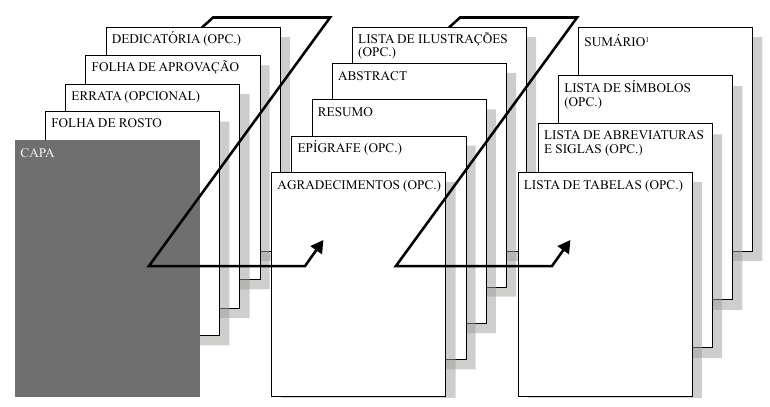
\includegraphics[width=0.6\textwidth]{figuras/pretextuais.png}
% 		\fonte{Adaptado de \citeonline{man:MDTUFSM2015}.}
% 	    \end{figure}
%          \end{verbatim}
         
%          \begin{figure}[ht]
%      	    \caption{\label{exepretex}Sequência dos elementros pré-testuais da MDT-UFSM.}
% 	    \centering
% 	    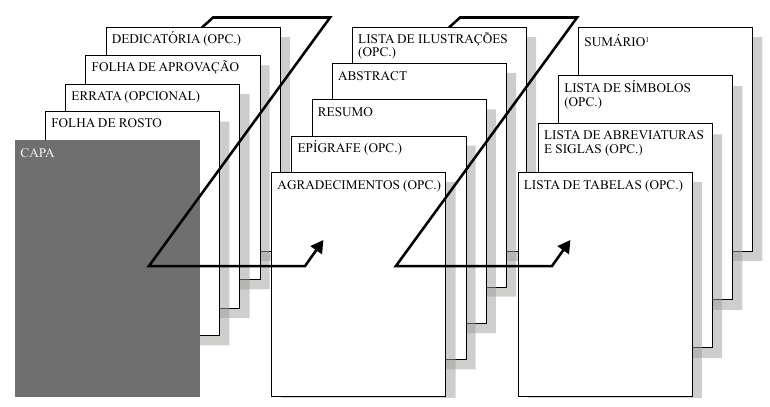
\includegraphics[width=0.6\textwidth]{figuras/pretextuais.png}
%             \fonte{Adaptado de \citeonline{man:MDTUFSM2015}.}
%          \end{figure}
        
% 	\par Para inserir ilustrações e gráficos, foram criados novos ambientes: ``ilustracao'' e ``grafico''. Estes ambientes são semelhantes ao ambiente ``figure'', porém geram sua própria lista. A seguir, exemplos da utilização nos novos ambientes.
	
% 	\begin{verbatim}
% 	    \begin{ilustracao}[ht]
% 		\caption{\label{exepretex1}Sequência dos elementros pré-testuais da MDT-UFSM}
%                 \centering
% 		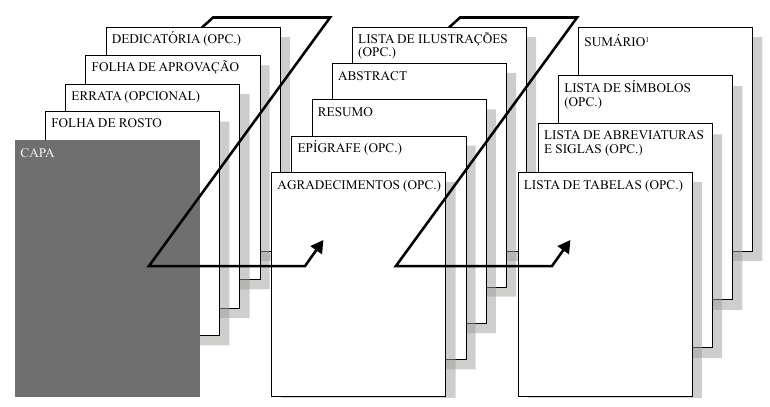
\includegraphics[width=0.6\textwidth]{figuras/pretextuais.png}
% 		\fonte{Adaptado de \citeonline{man:MDTUFSM2015}.}
% 	    \end{ilustracao}
%          \end{verbatim}
         
%          \begin{ilustracao}[ht]
%      	    \caption{\label{exepretex1}Sequência dos elementros pré-testuais da MDT-UFSM.}
% 	    \centering
% 	    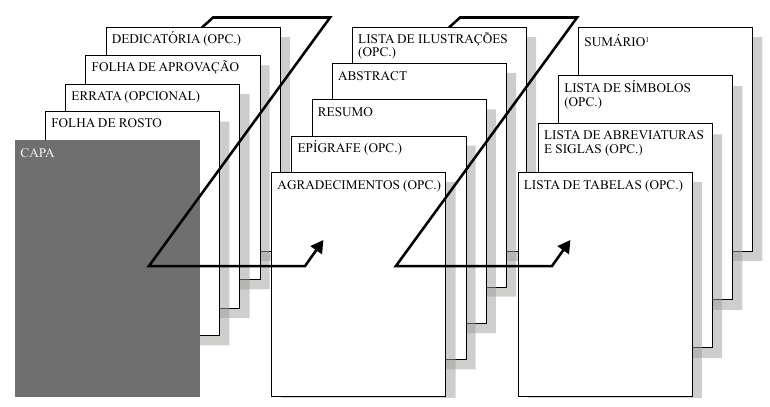
\includegraphics[width=0.6\textwidth]{figuras/pretextuais.png}
%             \fonte{Adaptado de \citeonline{man:MDTUFSM2015}.}
%          \end{ilustracao}
	
         
% 	\begin{verbatim}
% 	    \begin{grafico}[ht]
% 		\centering
% 		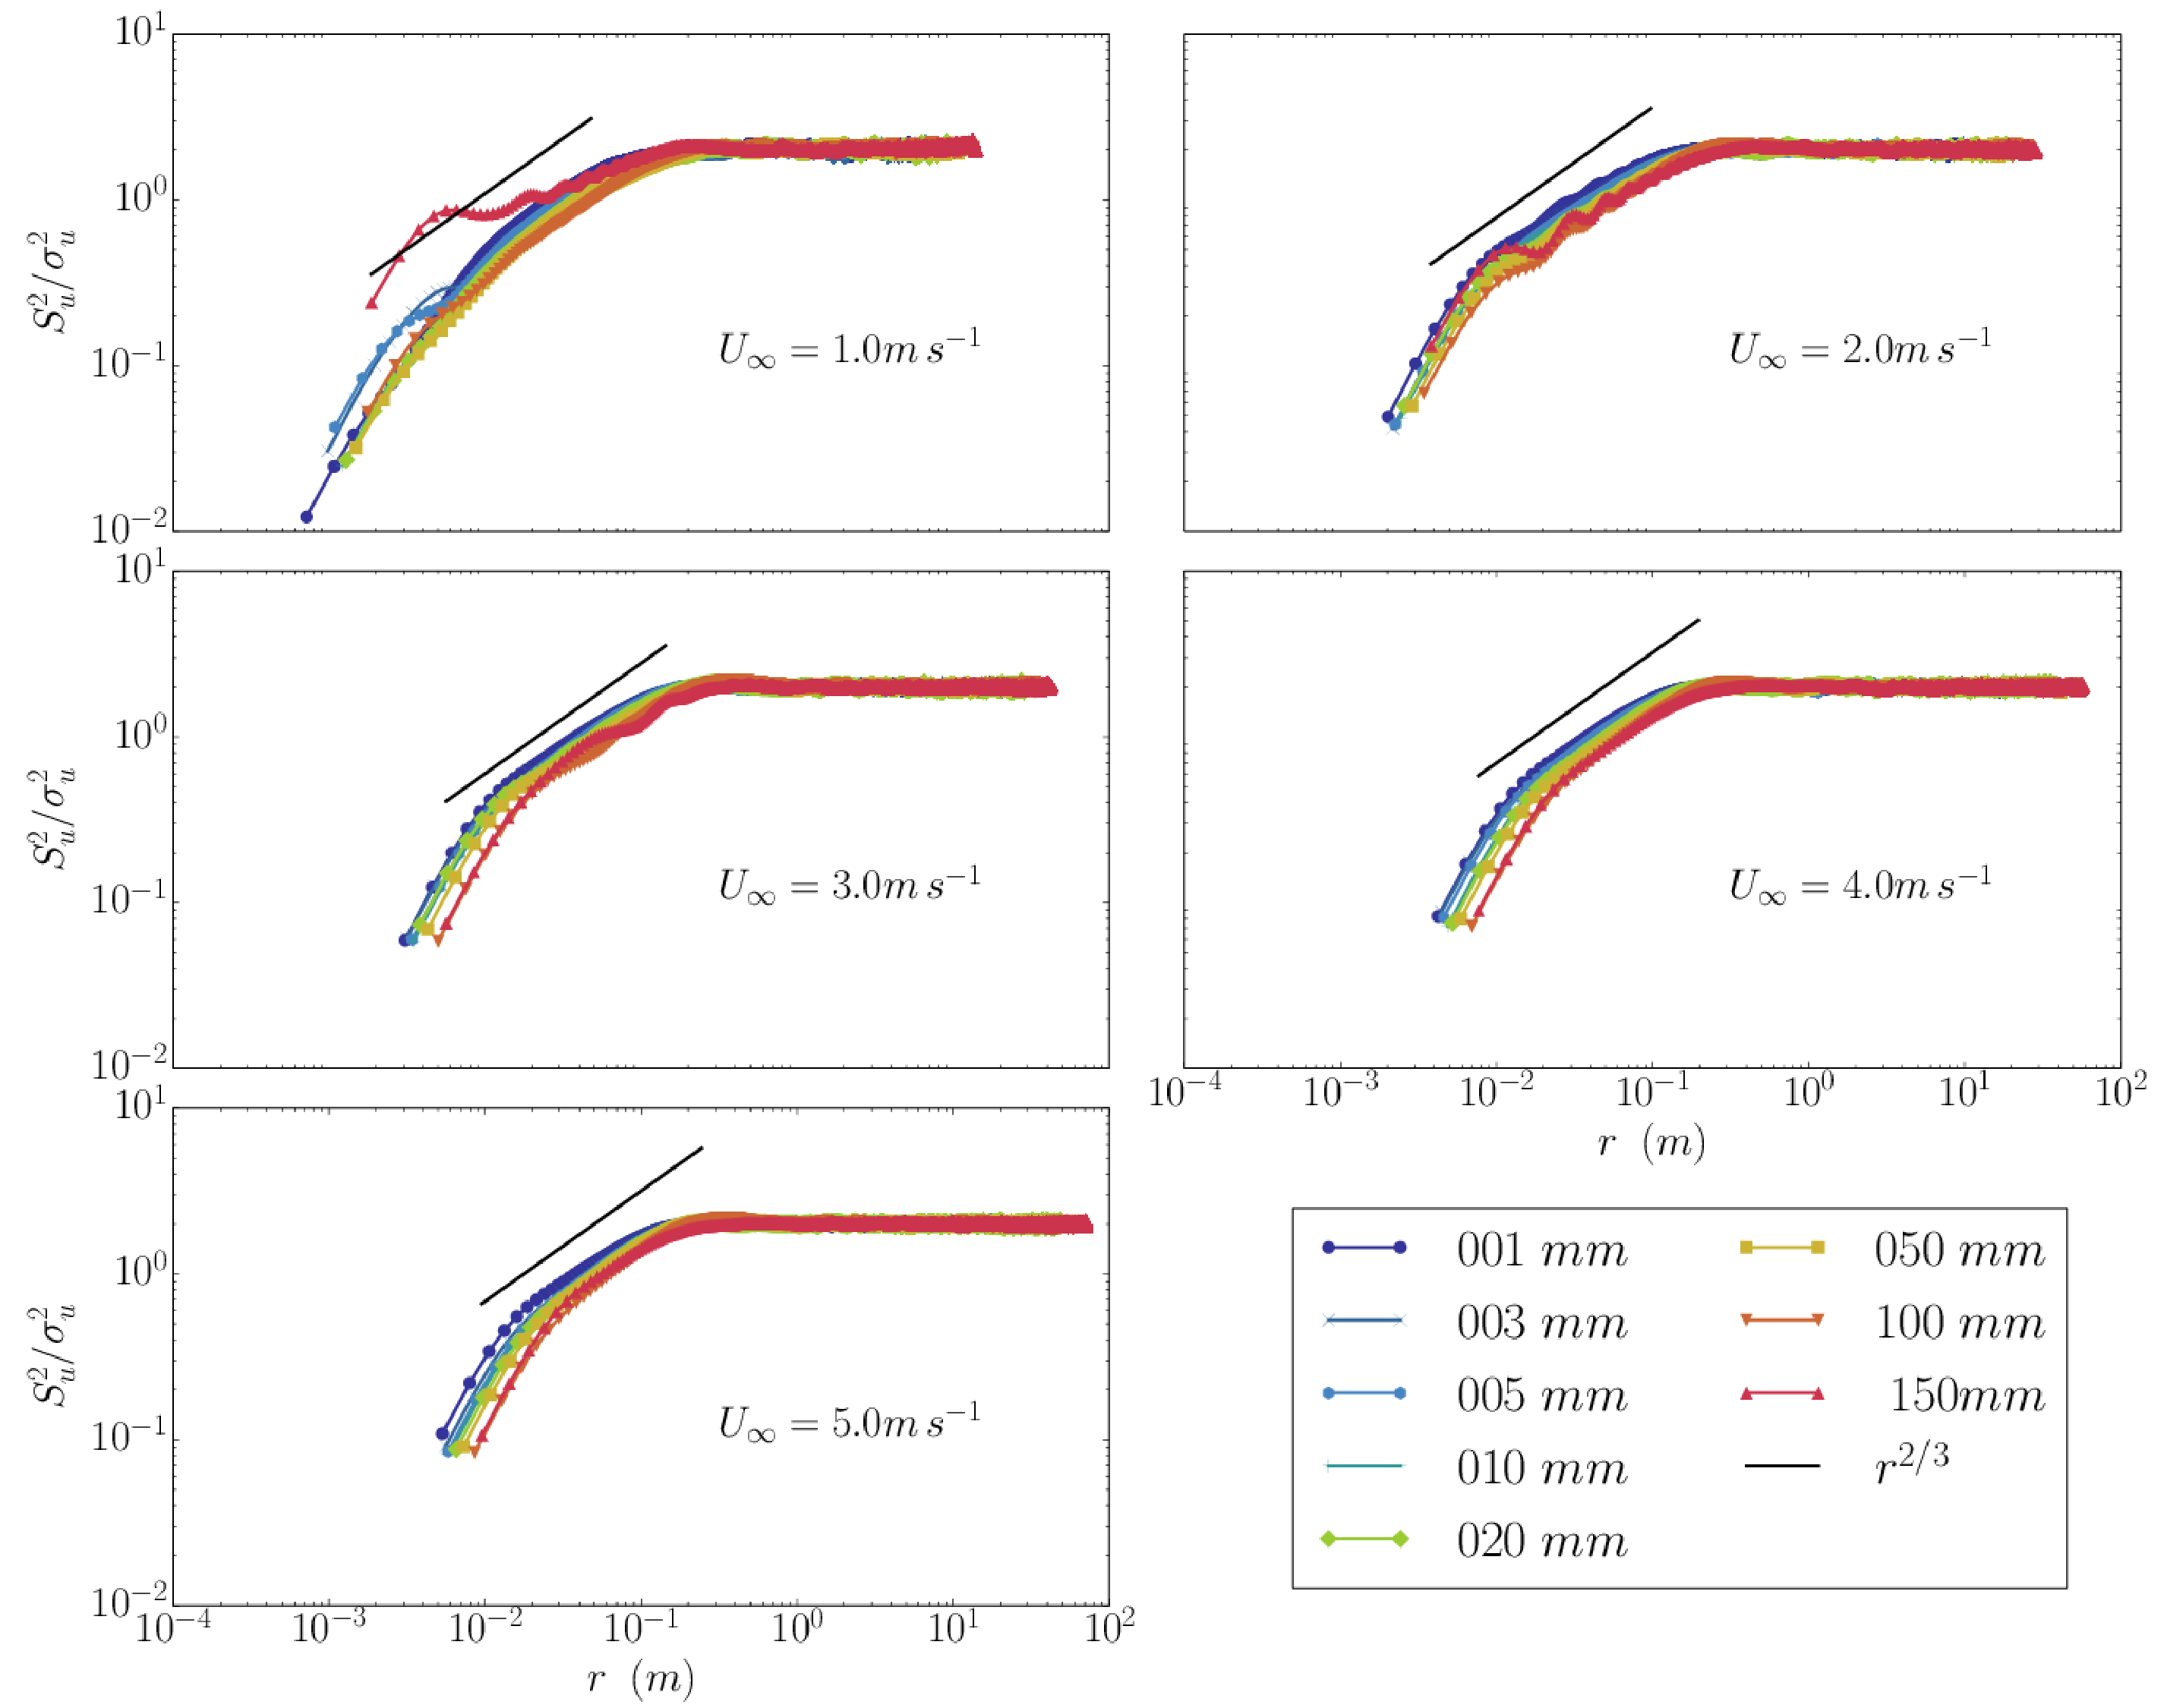
\includegraphics[width=0.6\textwidth]{figuras/estrutura_com.pdf}
% 		\caption{\label{exepretex3} Um exemplo de utilização do ambiente ``grafico''.}
% 		\fonte{Próprio autor.}
% 	    \end{grafico}
%          \end{verbatim}
         
% 	    \begin{grafico}[ht]
% 	\caption{\label{exepretex3}Um exemplo de utilização do ambiente ``grafico''.}
%              \centering
% 		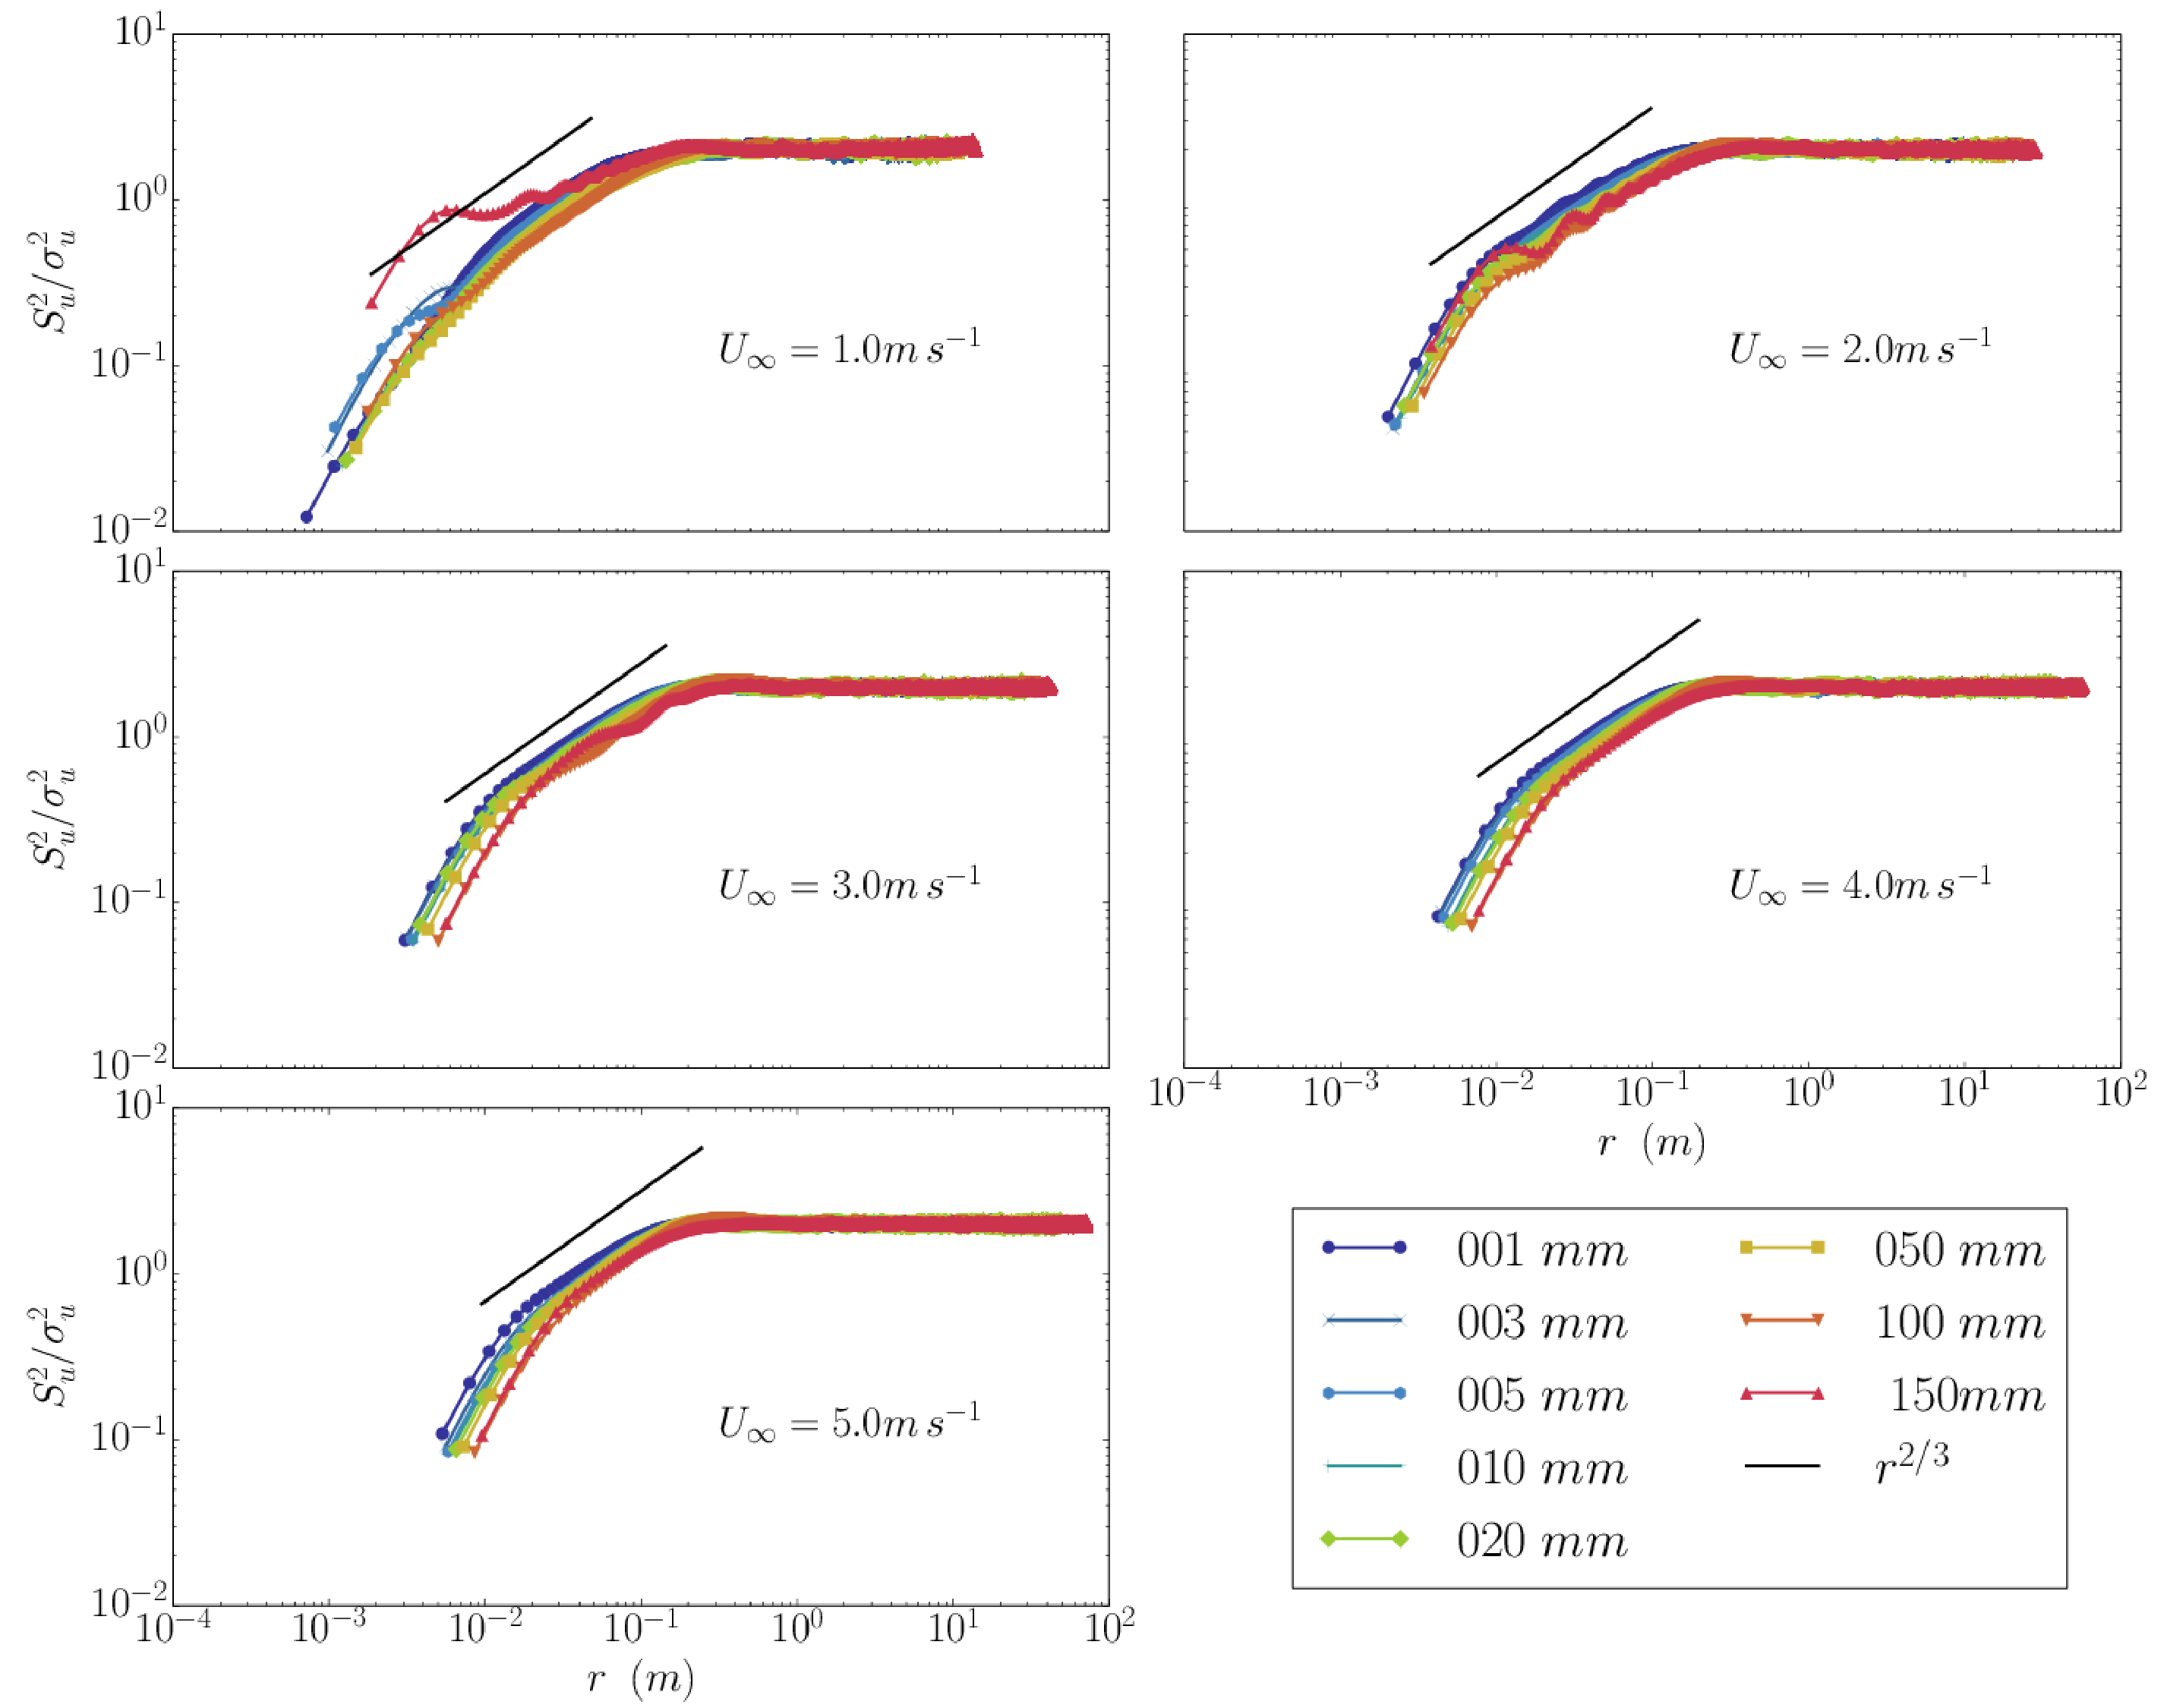
\includegraphics[width=0.6\textwidth]{figuras/estrutura_com.pdf}
% 		\fonte{Próprio autor.}
% 	    \end{grafico}
         
% \chapter{Conclusão}

% 	\par Conclusão do trabalho.
% 	\lipsum[1-5]


	
	
% % % % % % % % % % % % % % % % % % % % % % % % % % % % % % % % % % % % % % 
% % % % % % % % % % % % FIM DAS PAGINAS TEXTUAIS % % % % % % % % % % % % % % 
% % % % % % % % % % % % % % % % % % % % % % % % % % % % % % % % % % % % % % 



% % % % % % % % % % % % % % % % % % % % % % % % % % % % % % % % % % % % % % 	
% % % % % % % % % % % % % BIBLIOGRAFIA  % % % % % % % % % % % % % % % % % % 
% % % % % % % % % % % % % % % % % % % % % % % % % % % % % % % % % % % % % % 	

\startbibliography % comando para formatar na MDT UFSM
\bibliography{referencias}

	
% % % % % % % % % % % % % % % % % % % % % % % % % % % % % % % % % % % % % 	
% % % % % % % % % % % % % APENDICES % % % % % % % % % % % % % % % % % % %
% % % % % % % % % % % % % % % % % % % % % % % % % % % % % % % % % % % % % 	
% \apendice %%%% TEXTOS A PARIR DESTE PONTO SERAO CONSIDERADOS APENDICES

% \chapter{Demonstração de algo}
%         \par Algo como apêndice.  
%          \lipsum[2-10]

          
% % % % % % % % % % % % % % % % % % % % % % % % % % % % % % % % % % % % % % 	
% % % % % % % % % % % % % % % ANEXOS  % % % % % % % % % % % % % % % % % % % 
% % % % % % % % % % % % % % % % % % % % % % % % % % % % % % % % % % % % % % 	
        % \anexo    %%%% TEXTOS A PARIR DESTE PONTO SERAO CONSIDERADOS ANEXOS
        
% \chapter{Algo interessante que alguém fez}
%          \par Algo como anexo.
%          \lipsum[2-10]
                  
%         \begin{grafico}[ht]
%      	    \caption{\label{exepretex2}Orientações para a lombada do trabalho.}
% 	    \centering
% 	    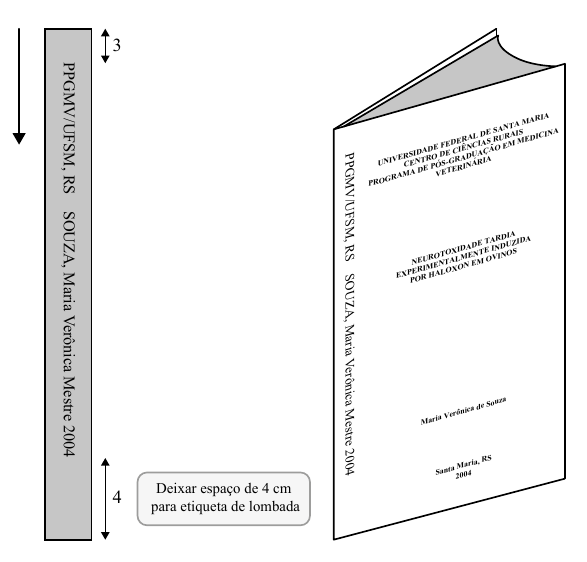
\includegraphics[width=0.6\textwidth]{figuras/lombada.png}
%             \fonte{Adaptado de \citeonline{man:MDTUFSM2015}.}
%          \end{grafico}         
         
%          \lipsum[2-10]

      
         
\end{document}
